% !TEX root = perelman-geometry.tex
%!TEX TS-program = pdflatex
%!TEX encoding = UTF-8 Unicode

% epigraph for part 1

\cleardoublepage
\vspace*{\fill}
\begin{center}
\epigraph{\begin{minipage}{0.4\pagewidth} \textsf{Nature speaks the language of mathematics: the letters of this language are circles, triangles and other mathematical shapes.}\end{minipage}}{Galileo}
\end{center}
\vspace*{\fill}

\thispagestyle{empty}

% begin chapter

\cleardoublepage

%\RedeclareSectionCommand[beforeskip=2.75cm]{chapter}
%\RedeclareSectionCommand[afterskip=1cm]{chapter}
%\RedeclareSectionCommand[beforeskip=0.1\baselineskip,afterskip=0.25\baselineskip]{section}
%
%\RedeclareSectionCommand[beforeskip=-1cm]{section}
%\vspace*{2cm} % Adjust the value as needed

\setchapterpreamble[o]{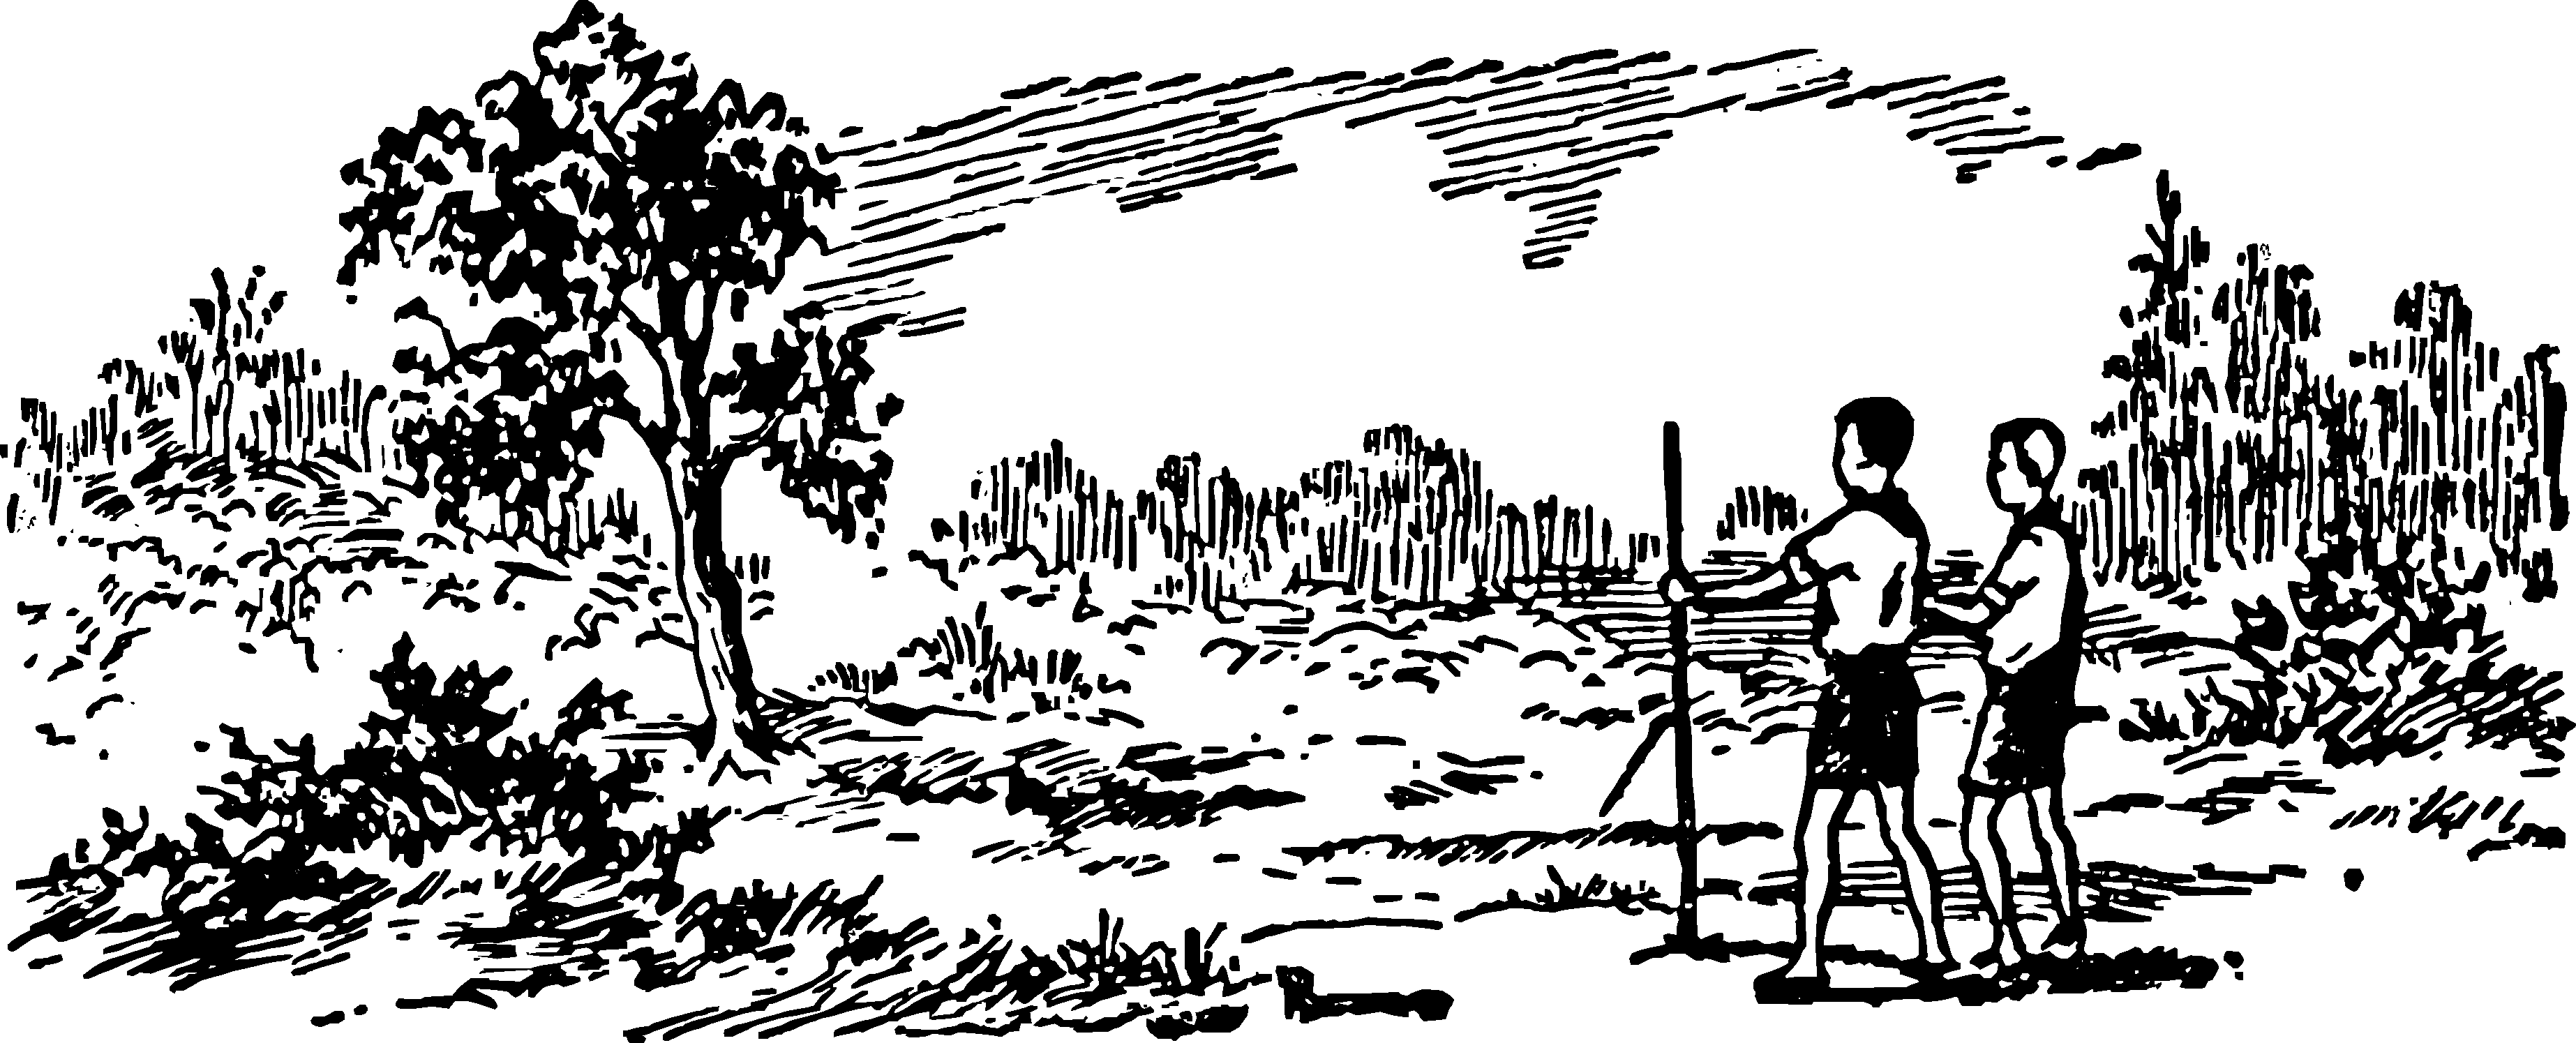
\includegraphics[width=1.2\textwidth]{figures/ch-01/fig-ch-01-head.pdf}\bigskip}

\chapter{Geometry In The Forest}
\label{ch-01}

%\begin{tikzpicture}[remember picture,overlay,shift=(current page.north west)]
%\begin{scope}[x={(current page.north east)},y={(current page.south west)}]
%\node [overlay,remember picture] at (0.5,0.2) {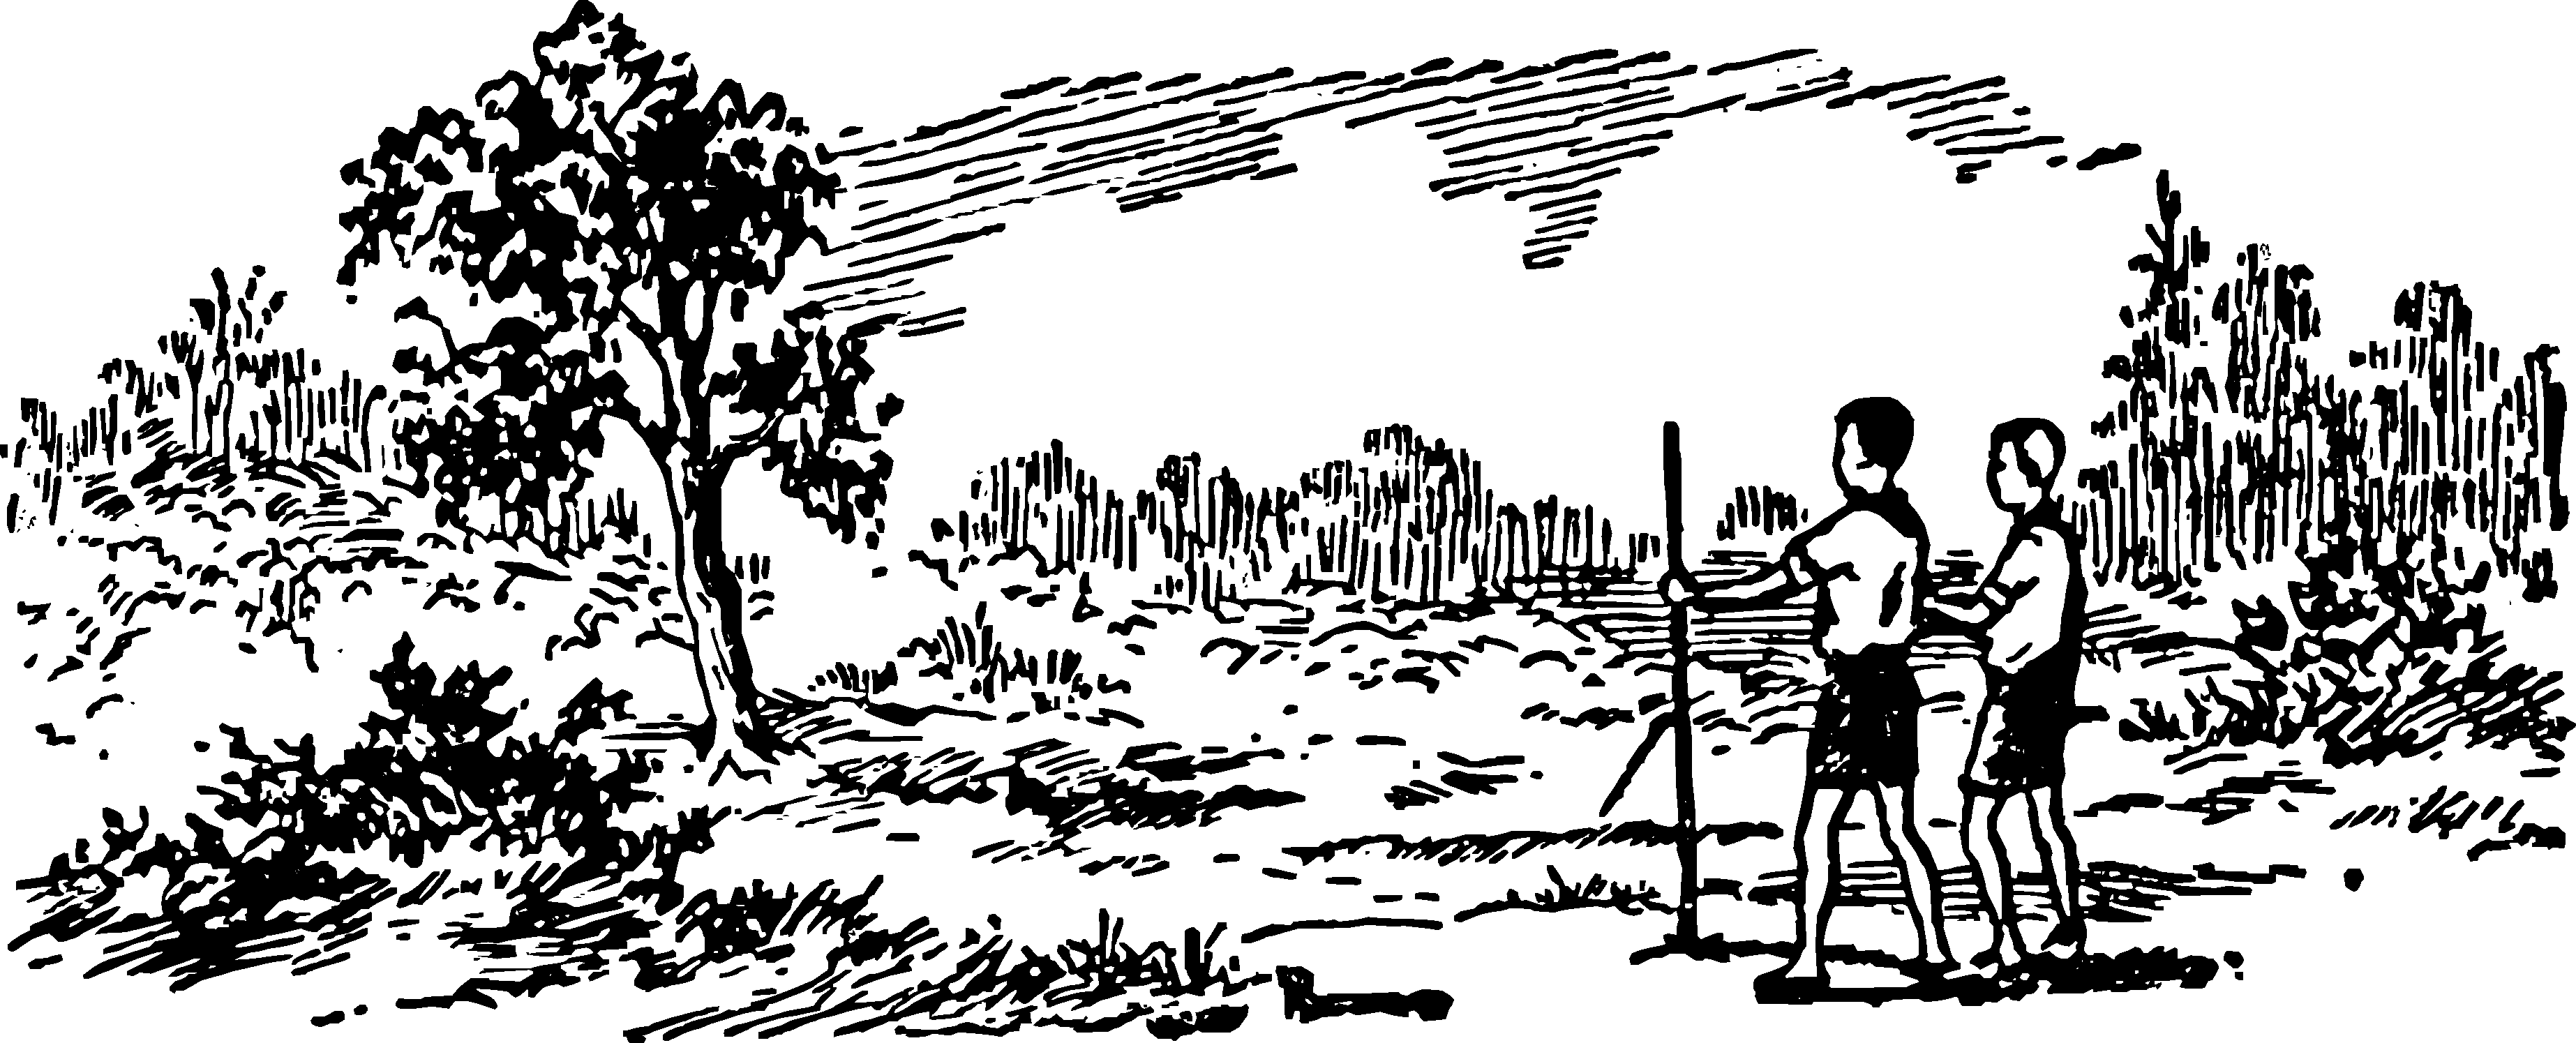
\includegraphics[width=1.2\textwidth]{figures/ch-01/fig-ch-01-head.pdf}};
%\end{scope}
%\end{tikzpicture}

\section{By the length of the shadow}
\label{sec-1.1}

I remember now the amazement with which I looked

for the first time, he looked at a gray-haired forester, who, standing near a huge pine tree, measured its height with a small pocket device. When he aimed his square board at the top of the tree, I expected that the old man would now start climbing there with a measuring chain. Instead, he put the device back in his pocket and announced that the measurement was over. I thought it hadn't started yet \ldots{}

I was very young then, and this way of measuring, when a person determines the height of a tree without cutting it down and climbing to the top, was in my eyes something like a small miracle. It was only later, when I was initiated into the rudiments of geometry, that I realised how simple such miracles are performed. There are many different ways to make such measurements using very simple instruments and even without any devices.

The easiest and most ancient way is, without a doubt, the one by which the Greek sage Thales determined the height of the pyramid in Egypt sixth century BC. He took advantage of the pyramid's `shadow'. The priests and the pharaoh, gathered at the foot of the highest pyramid, looked puzzled at the northern newcomer, who guessed the height of the huge structure from the shadow. Thales, says the legend, chose a day and an hour when the length of his own shadow was equal to his height; at this moment, the height of the pyramid should also be equal to the length of the shadow cast by it\sidenote{Of course, the length of the shadow had to be measured from the midpoint of the square base of the pyramid; Thales could directly measure the width of this base.}. This is perhaps the only case when a person benefits from his shadow \ldots{}

The task of the Greek sage now seems childishly simple to us, but let's not forget that we are looking at it from the height of a geometric building erected after Thales. He lived long before Euclid, the author of the wonderful book that taught geometry for two millennia after his death. The truths contained in it, which are now known to every schoolboy, were not yet discovered in the era of Thales. And in order to use the shadow to solve the problem of the height of the pyramid, it was necessary to already know some geometric properties of the triangle, namely the following two (of which Thales himself discovered the first):
\begin{enumerate}
\item that the angles at the base of an isosceles triangle are equal, and vice versa -- that the sides lying opposite the equal angles of the triangle are equal to each other;
\item that the sum of the angles of any triangle (or at least a rectangular one) is equal to two right angles.
\end{enumerate}

Only Thales, armed with this knowledge, had the right to conclude that when his own shadow is equal to his height, the sun's rays meet the flat ground at an angle of half a straight line, and therefore the top of the pyramid, the middle of its base and the end of its shadow should mark an isosceles triangle.

It would seem that this simple method is very convenient to use on a clear sunny day to measure lonely trees whose shadow does not merge with the shadow of neighbouring ones. But in our latitudes it is not as easy as in Egypt to waylay the right moment for this: The sun is low above the horizon, and the shadows are equal to the height of the objects casting them only in the afternoon hours of the summer months. Therefore, the Thales method in this form is not always applicable.

\begin{figure}[h!]
\centering
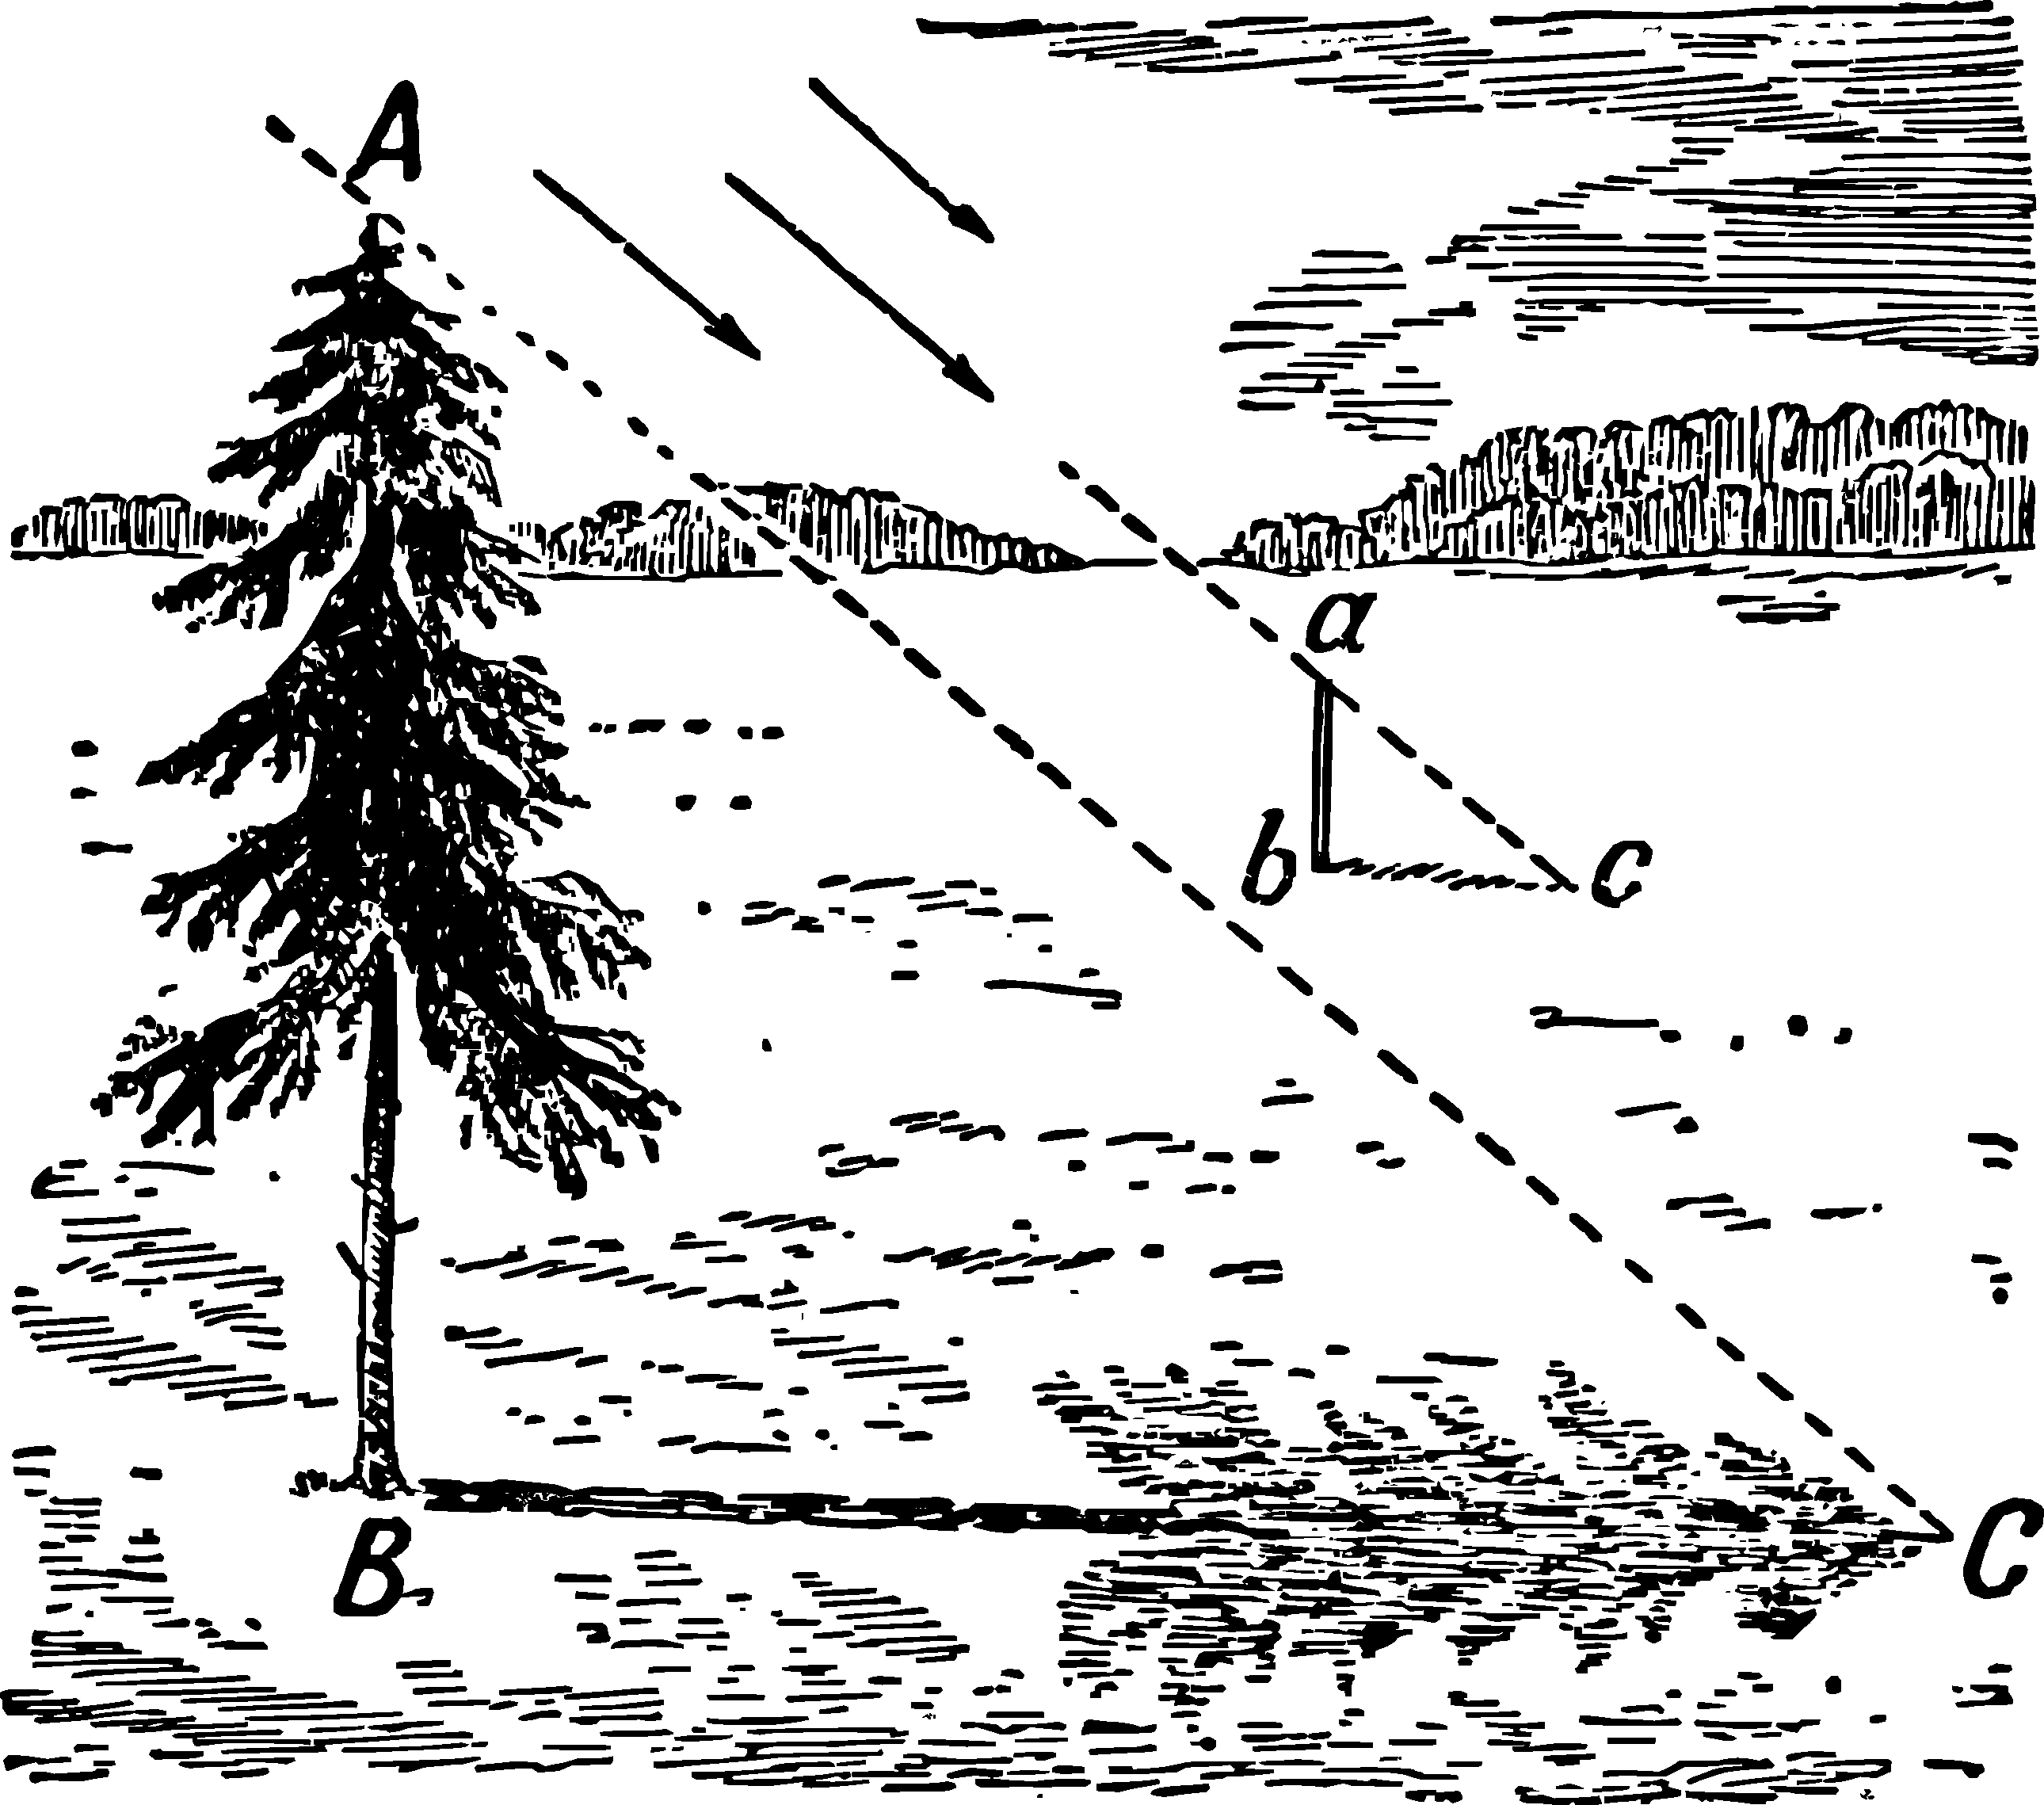
\includegraphics[width=0.9\textwidth]{figures/ch-01/fig-01-01.pdf}
\sidecaption{Measuring the height of a tree by shadow.\label{fig-01-01}}
\end{figure}
It is not difficult, however, to modify this method so that on a sunny day, any shadow can be used, regardless of its length. Additionally, measuring both your own shadow and the shadow of a pole, the desired height is calculated from the proportion (\figr{fig-01-01}):
\begin{equation*}%
AB:ab = BC:bc,
\end{equation*}
meaning the height of the tree is as many times greater than your own height (or the height of the pole) as the shadow of the tree is longer than your shadow (or the shadow of the pole). This naturally follows from the geometric similarity of triangles $ABC$ and $abc$ (based on two angles).

Some readers may object that such an elementary technique does not need a geometric justification at all: is it really unclear even without geometry that how many times is a tree taller, how many times is its shadow longer? However, the matter is not as simple as it seems. Try to apply this rule to shadows cast by the light of a street lamp or lamp -- it will not be justified. In \figr{fig-01-02} you can see that the columns $AB$ are about three times higher than the pedestal $ab$, and the shadow of the column is eight times larger than the shadow of the pedestal $(BC:bc)$. It is impossible to explain why the method is applicable in this case, but not in the other, without geometry.

\begin{figure}[h!]
\centering
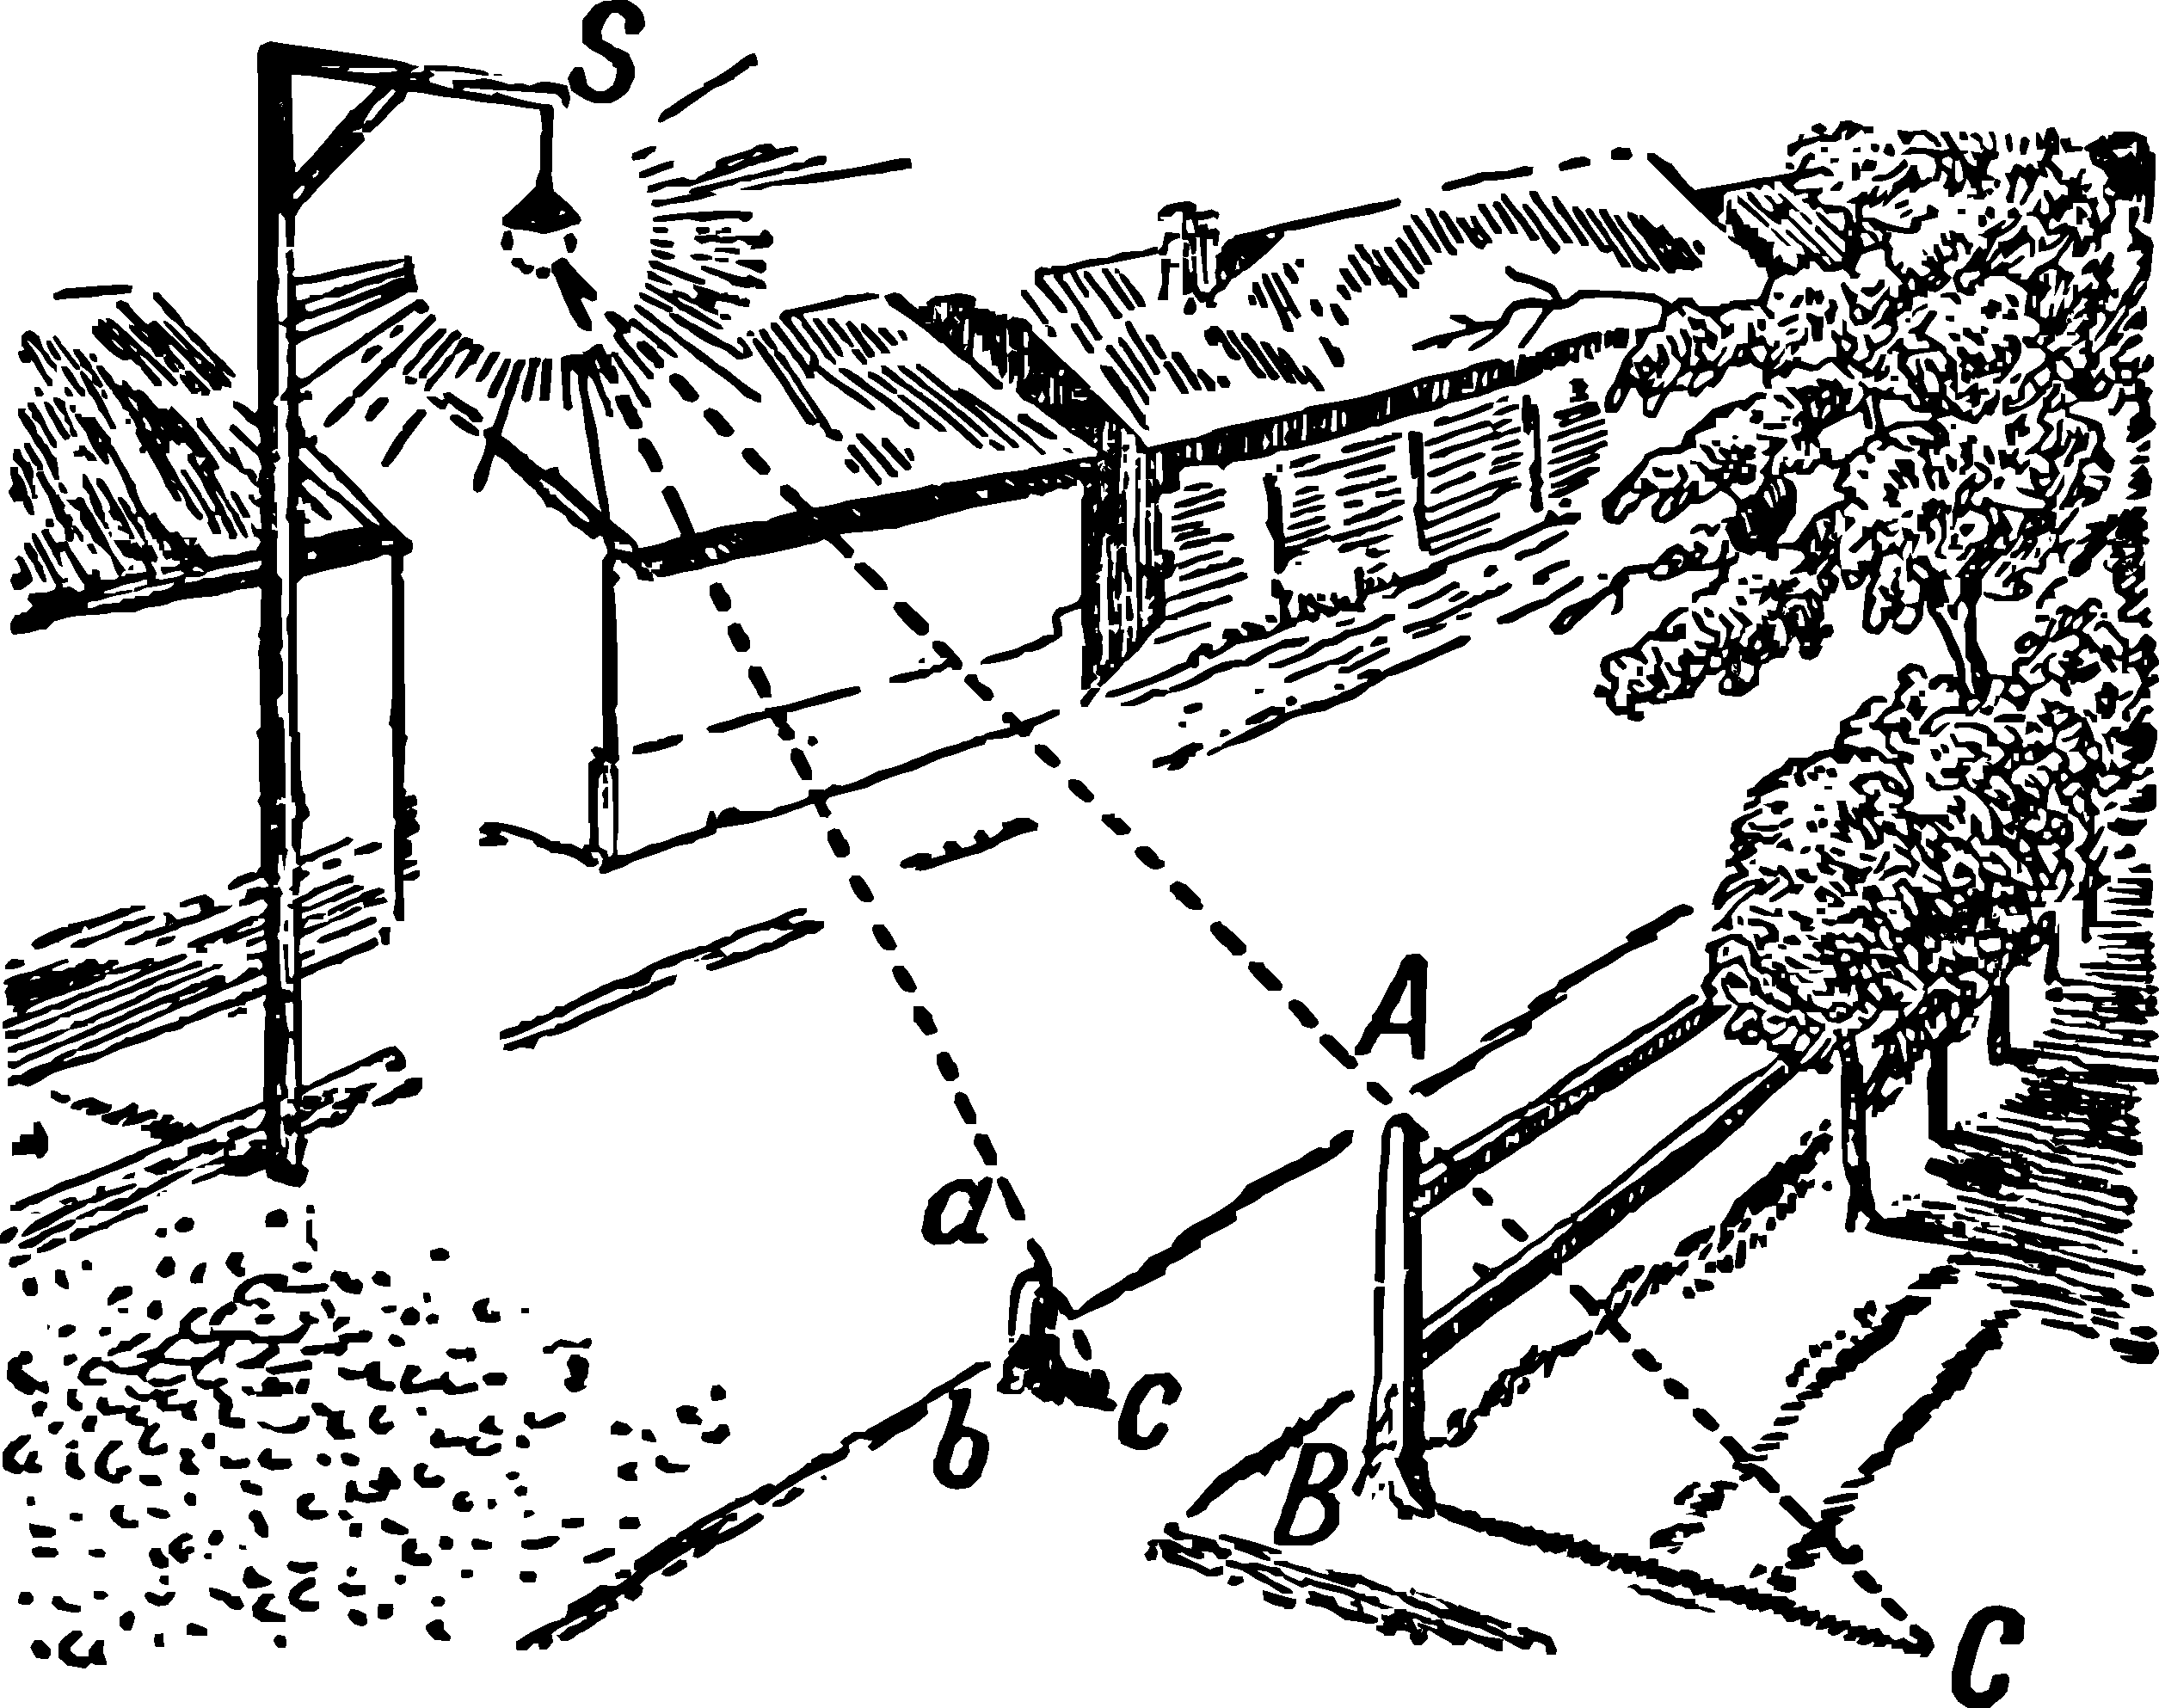
\includegraphics[width=0.9\textwidth]{figures/ch-01/fig-01-02.pdf}
\sidecaption{When such a measurement is impossible. (Is the method applicable for a shadow cast by a streetlamp?)\label{fig-01-02}}
\end{figure}

\subsection*{Question}

Let's take a closer look at what the difference is. The essence of the matter boils down. to the fact that the sun's rays are parallel to each other, the rays of the lantern are not parallel. After that, we have the right to consider the rays of the Sun parallel, although they certainly intersect in the place from which they originate.

\subsection*{Answer}

The rays of the Sun falling on the Earth can be considered parallel because the angle between them is extremely small, almost imperceptible. A simple geometric calculation will convince you of this. Imagine two rays coming from some point of the Sun and falling on the Earth at a distance of, say, one kilo-meter from each other. So, if we put one leg of a compass at this point of the Sun, and with the other we described a circle with a radius equal to the distance from the Sun to the Earth (i.e., with a radius of \SI{150000000}{\kilo\meter}), then an arc of one kilometer in length would appear between our two radii rays. The total length of this gigantic circle would be equal to $2 \pi \times \SI{150000000}{\kilo\meter} = \SI{940000000}{\kilo\meter}$. One degree of it, of course, is 360 times less, i.e. about \SI{2600000}{\kilo\meter}; one arc minute is 60 times less than a degree, i.e. equal to \SI{43000}{\kilo\meter}, and one arc second is another 60 times less, i.e. \SI{720}{\kilo\meter}. But our arc is only \SI{1}{\kilo\meter} in length, so it corresponds to an angle of $1/720 \approx \ang{;;0.00138}$ seconds. This angle is elusive even for the most accurate astronomical instruments; therefore, in practise we can consider the rays of the Sun falling on the Earth as parallel lines.\sidenote{Another thing is the rays directed from some point of the Sun to the ends of the earth's diameter; the angle between them is large enough to measure (about \ang{;;17}); the definition of this angle gave astronomers one of the means to establish how great the distance from the Earth to the Sun is.}

Trying to apply the method of shadows in practise, you will immediately be convinced, however, of its unreliability. Shadows are not delimited so clearly that measuring their length can be done quite accurately. Each shadow cast by the light of the Sun has an indistinctly outlined grey border of penumbra, which gives the border of the shadow uncertainty. This is because the Sun is not a point, but a large luminous body emitting rays from many points. \figr{fig-01-03} illustrates why, as a result of this, the shadow of tree $AB$ also has an additional component in the form of half-shadow $CD$, gradually fading away.

\begin{figure}[h!]
\centering
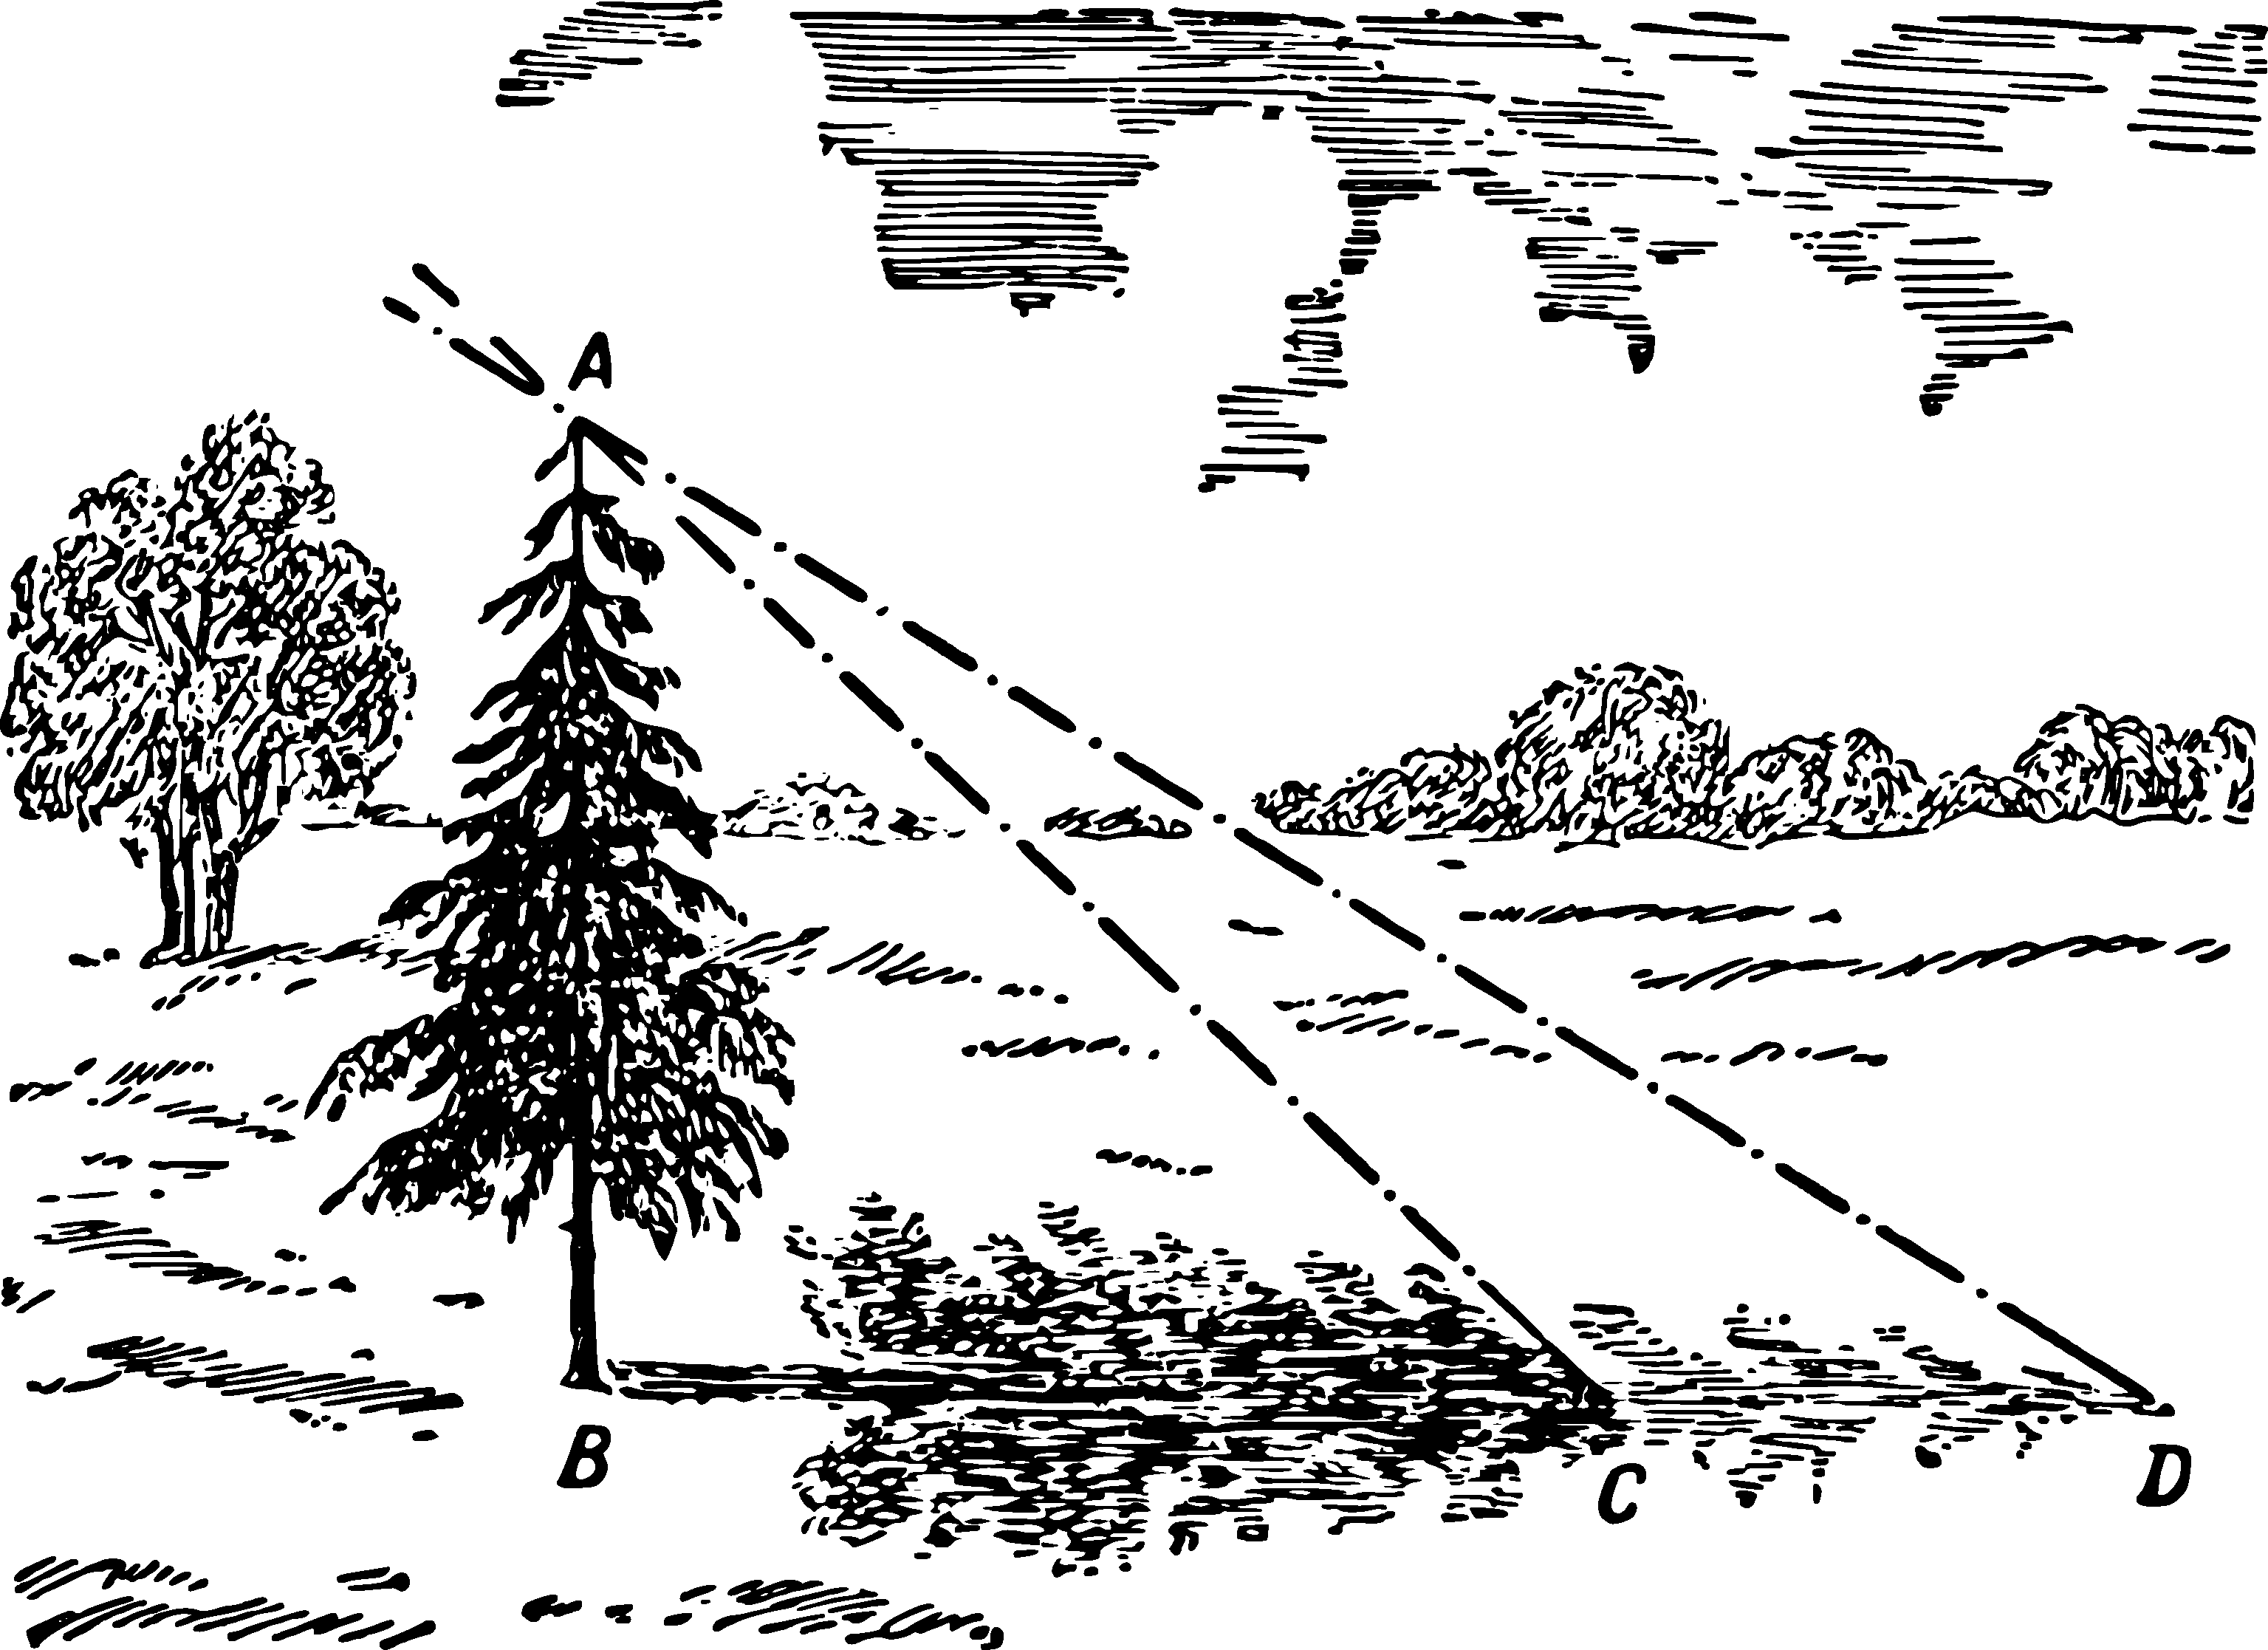
\includegraphics[width=0.9\textwidth]{figures/ch-01/fig-01-03.pdf}
\sidecaption{How penumbra is formed.\label{fig-01-03}}
\end{figure}


The angle of the $CAD$ between the extreme boundaries of the penumbra is equal to the angle at which we always see the solar disk, i.e. half a degree. The error resulting from the fact that both shadows are not measured quite accurately can reach 5\% or more when the Sun is not too low. This error is added to other unavoidable errors -- from uneven soil, etc. -- and makes the final result little reliable. In mountainous terrain, for example, this method is completely inapplicable.

\section{Two More Methods}
\label{sec-1.2}

It is entirely possible to measure height without relying on shadows. There are many methods; let's start with two simple ones.

Firstly, we can utilise the properties of an isosceles right triangle. For this purpose, we can make use of a very simple tool, which can be easily crafted from a piece of board and three pins. On a board of any shape, even a piece of bark with a flat side, mark three points to form the vertices of a right triangle -- and insert a pin at each point (see \figr{fig-01-04}). Suppose you don't have a drafting triangle to construct a right angle, nor a compass to mark equal sides. In that case, fold any piece of paper once, and then fold it again across the first fold so that both parts of the first fold coincide -- and you'll obtain a right angle. The same piece of paper can be used instead of a compass to measure equal distances.

\begin{figure}[h!]
\centering
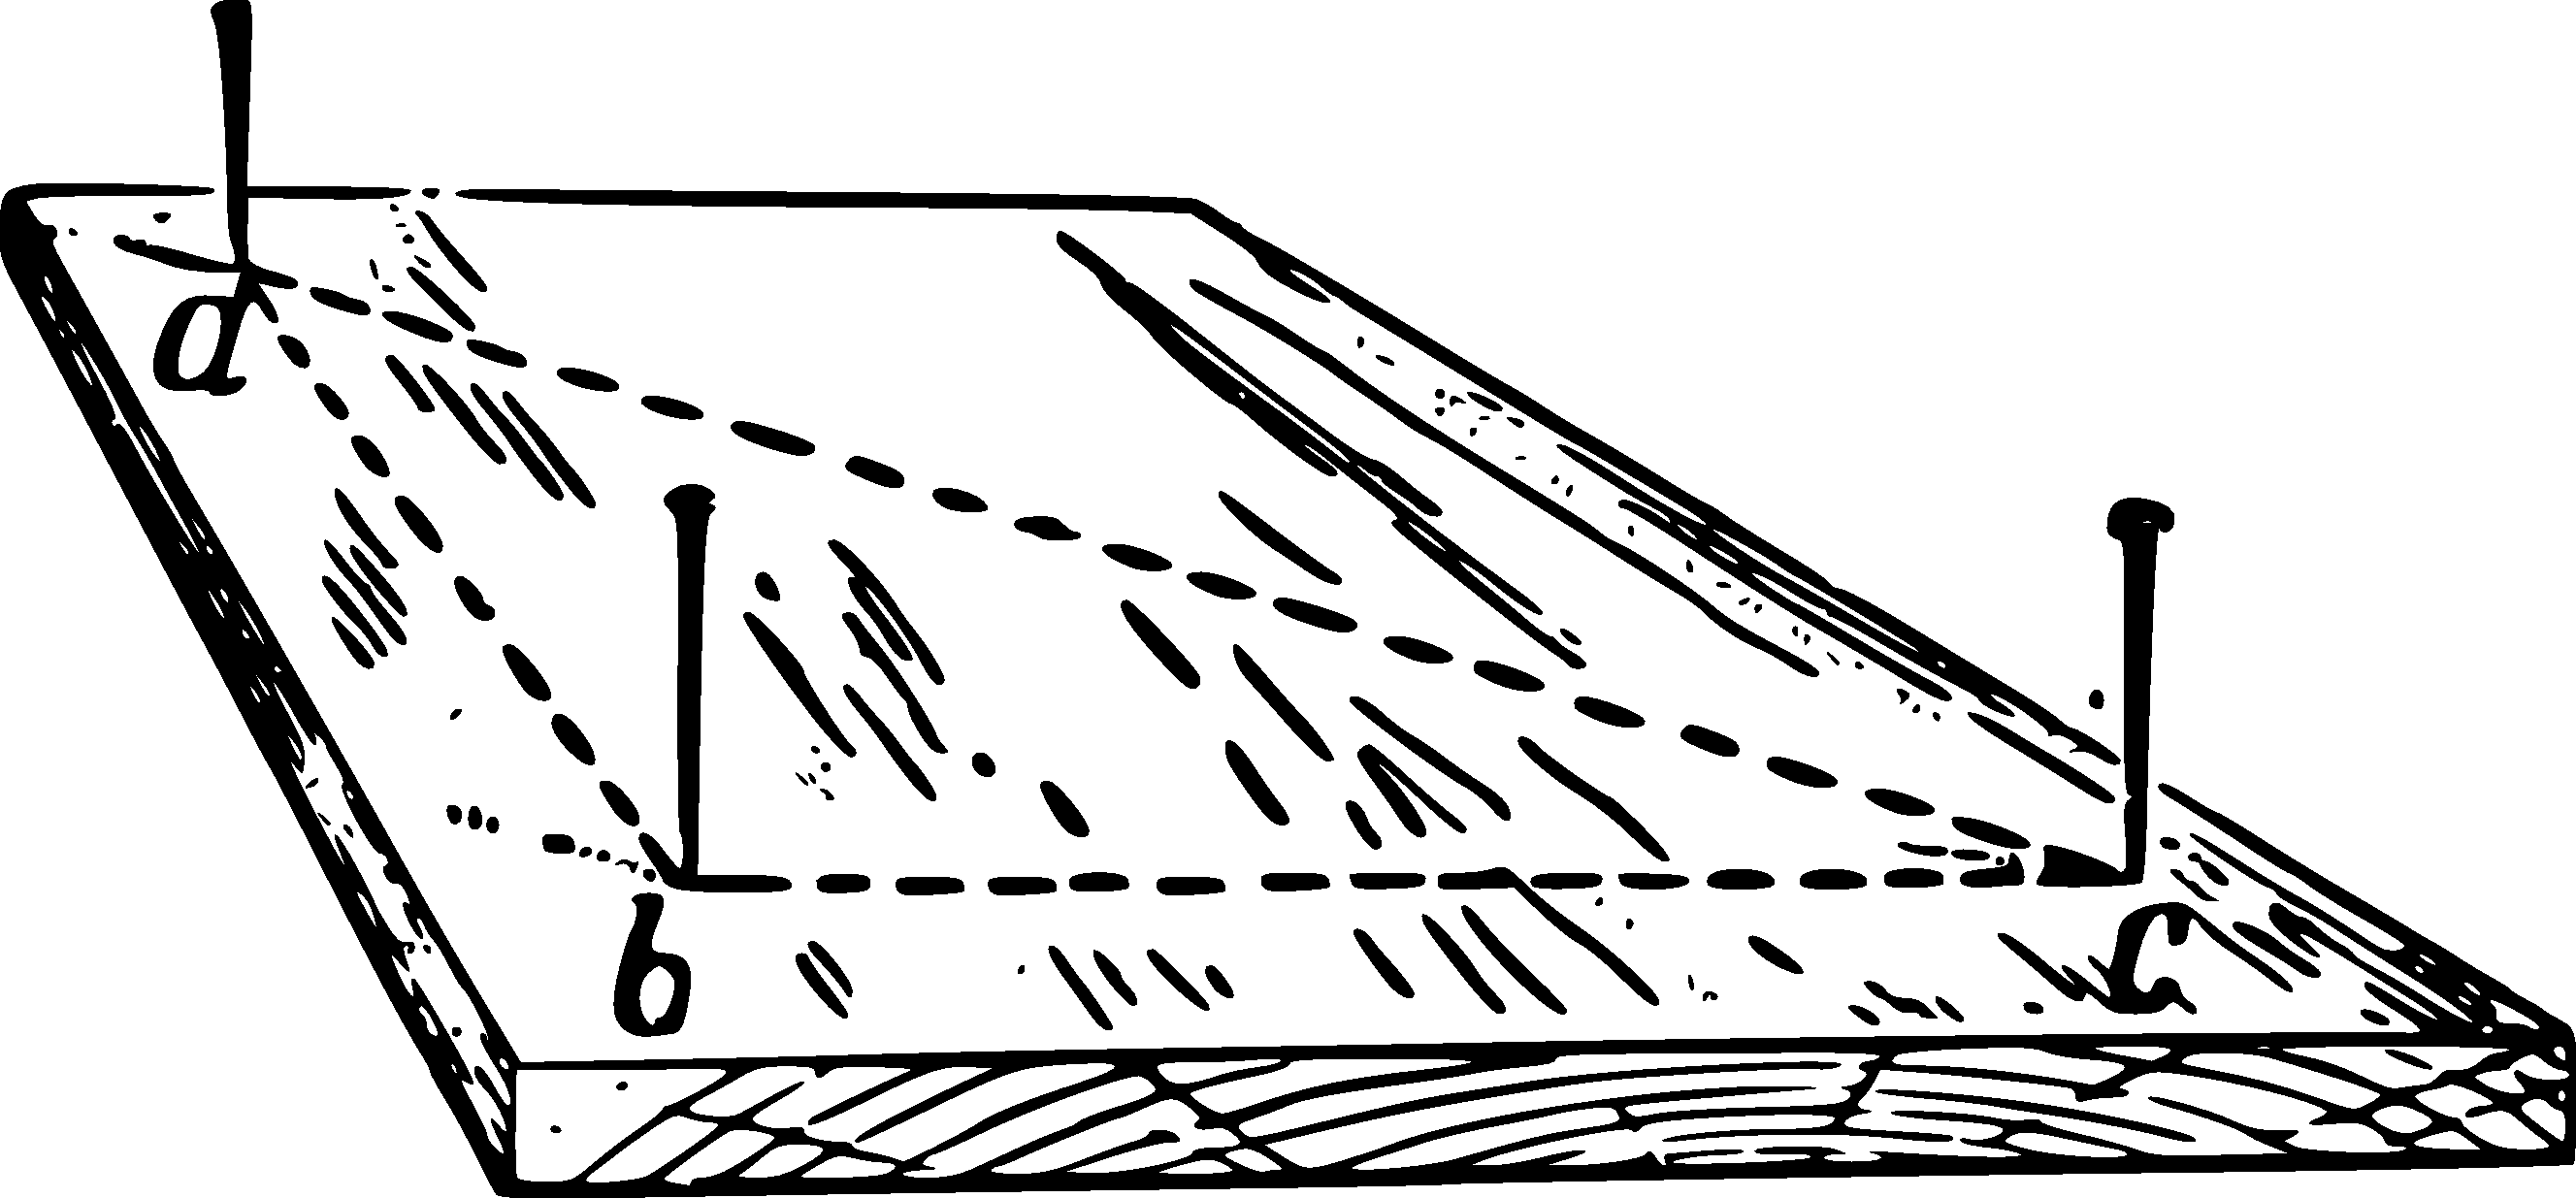
\includegraphics[width=0.6\textwidth]{figures/ch-01/fig-01-04.pdf}
\sidecaption{Pin height measuring device.\label{fig-01-04}}
\end{figure}


As you can see, the tool can be entirely crafted in a makeshift environment.

If you don't have a drafting triangle on hand to construct a right angle, nor a compass to mark equal sides, then simply fold any scrap of paper once, and then fold it again across the first fold so that both parts of the first fold coincide—and you'll obtain a right angle. The same piece of paper can be used instead of a compass to measure equal distances.

As you can see, the tool can be entirely crafted in a makeshift environment.

\begin{figure}[h!]
\centering
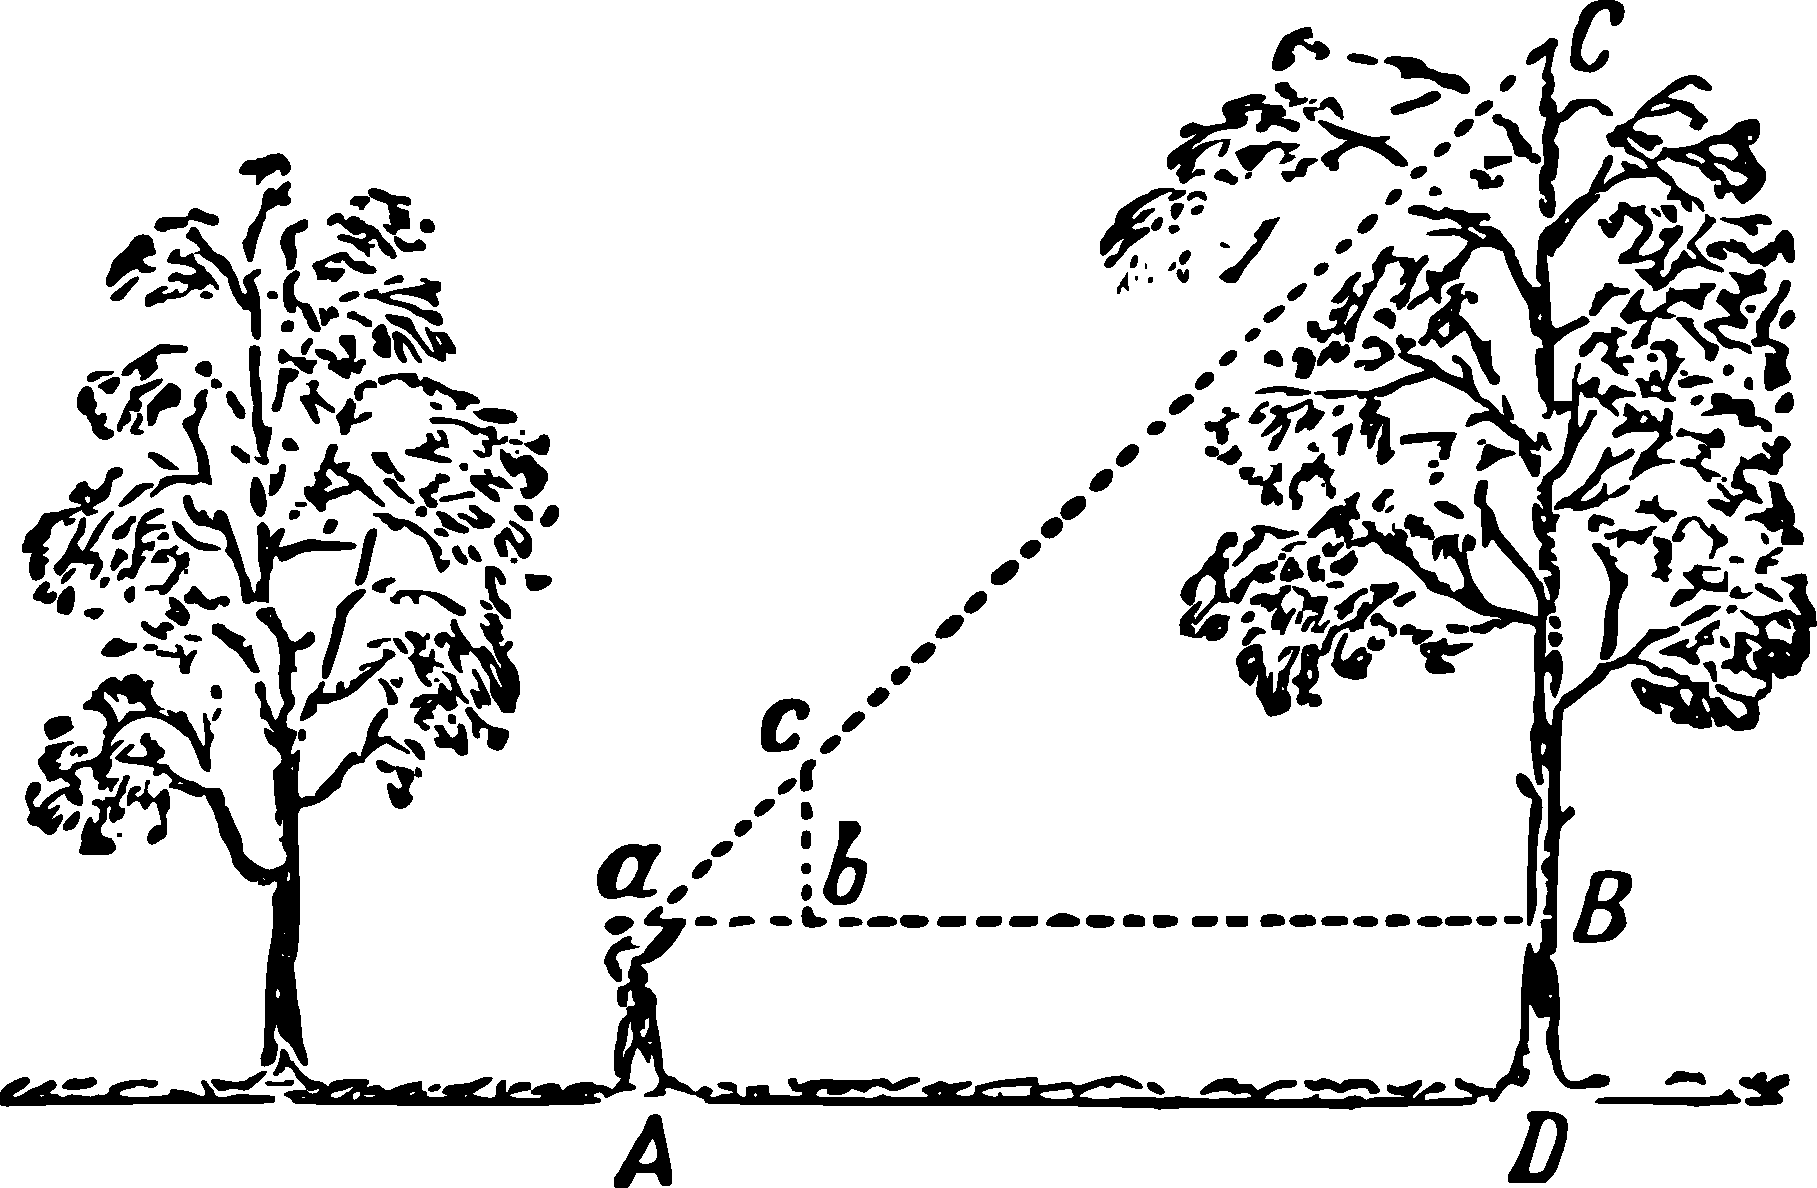
\includegraphics[width=0.9\textwidth]{figures/ch-01/fig-01-05.pdf}
\sidecaption{The scheme of application of the pin device.\label{fig-01-05}}
\end{figure}

Handling it is no more difficult than crafting it. Stepping away from the tree being measured, hold the tool so that one of the legs of the triangle is perpendicular. You can use a string or a weight tied to the top pin. Approaching or moving away from the tree, you will always find a spot $A$ (see \figr{fig-01-05}), from which, looking at pins $a$ and $c$, you will see that they cover the top $C$ of the tree: this means that the extension of the hypotenuse $ac$ passes through point $C$. Then, obviously, the distance $aB$ is equal to $CB$, since angle $a = \ang{45}$. 

Consequently, by measuring distance $aB$ (or, at another location, distance $AD$) and adding $BD$ to it, i.e., the elevation of point $a$ above the ground, you will obtain the desired height of the tree.

\begin{figure}[h!]
\centering
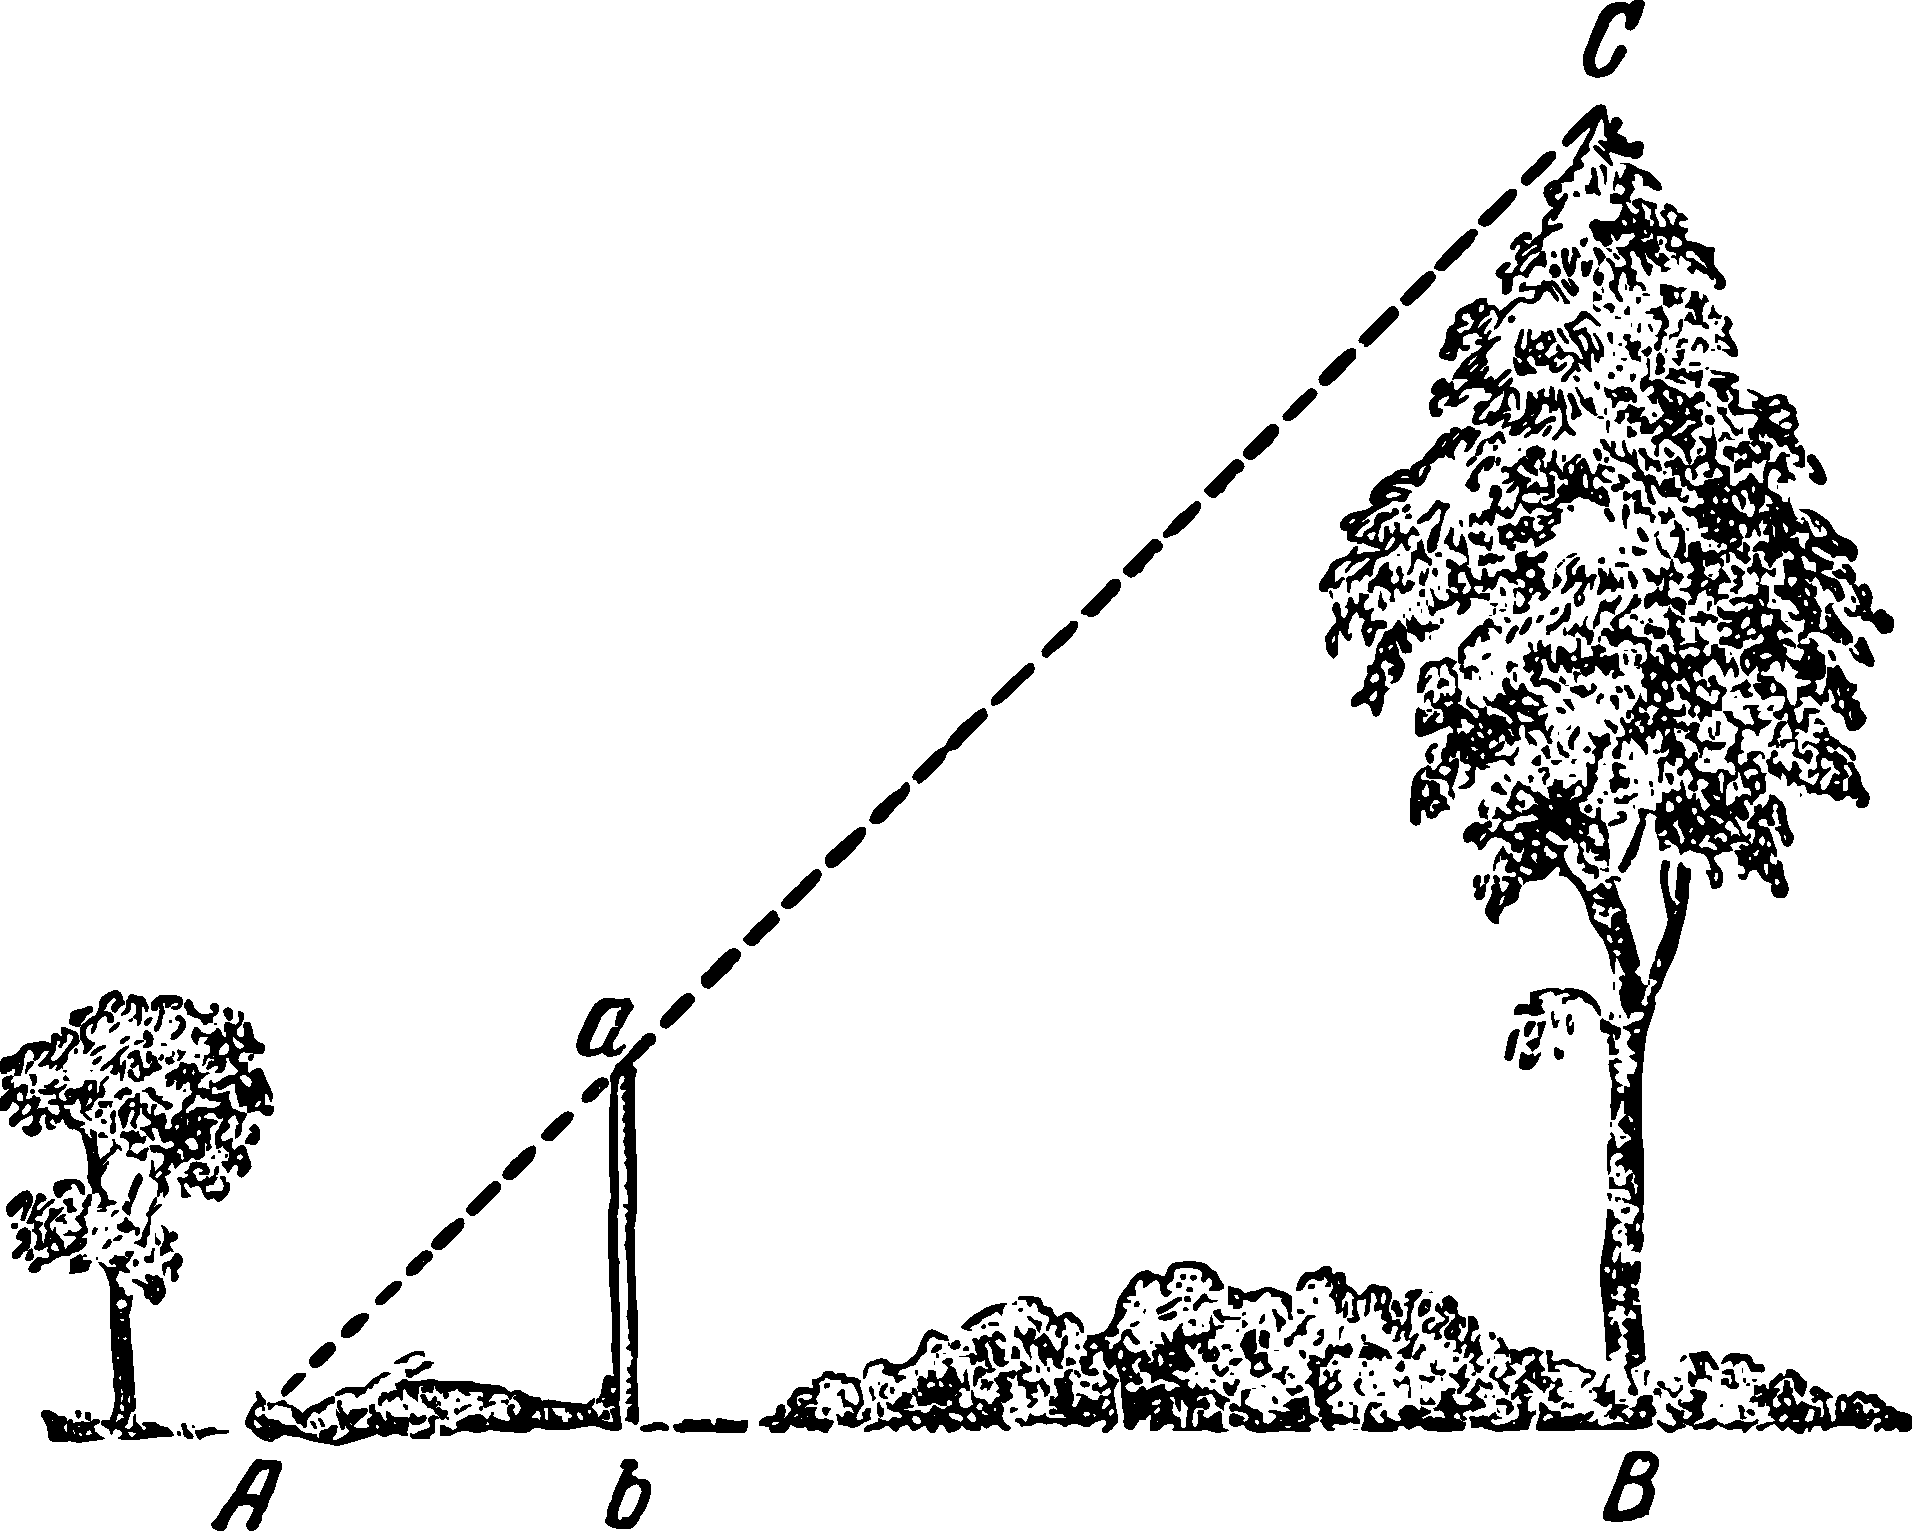
\includegraphics[width=0.9\textwidth]{figures/ch-01/fig-01-06.pdf}
\sidecaption{Another way to determine the height.\label{fig-01-06}}
\end{figure}

Another method does not even require a pin device. Here you need a pole, which you will have to insert vertically into the ground so that the protruding part is exactly at your height. The location for the pole must be chosen so that, lying down as shown in \figr{fig-01-06}, you see the top of the tree in a straight line with the upper point of the pole. Since triangle $Aba$ is isosceles and right-angled, angle $A = \ang{45}$, and therefore $AB$ equals $BC$, i.e., the desired height of the tree.



\section{The Method of Jules Verne}
\label{sec-1.3}

The next, also quite simple, method for measuring tall objects is vividly described by Jules Verne in his famous novel \emph{The Mysterious Island.}

``Today we need to measure the height of the Far View platform,'' said the engineer.

``Will you need a tool for that?'' asked Herbert.

``No, we won't. We'll proceed somewhat differently, resorting to a somewhat simpler and more accurate method.''

The young man, eager to learn as much as possible, followed the engineer, who descended from the granite wall to the rocky shore.

Taking a straight pole, twelve feet long, the engineer measured it as precisely as possible, comparing it to his own height, which he knew well. Meanwhile, Herbert held a plumb bob given to him by the engineer: just a stone attached to the end of a rope.

Not reaching five hundred feet from the granite wall, which rose vertically, the engineer drove the pole two feet into the sand and firmly secured it, placing it vertically with the help of the plumb bob.

\begin{figure}[h!]
\centering
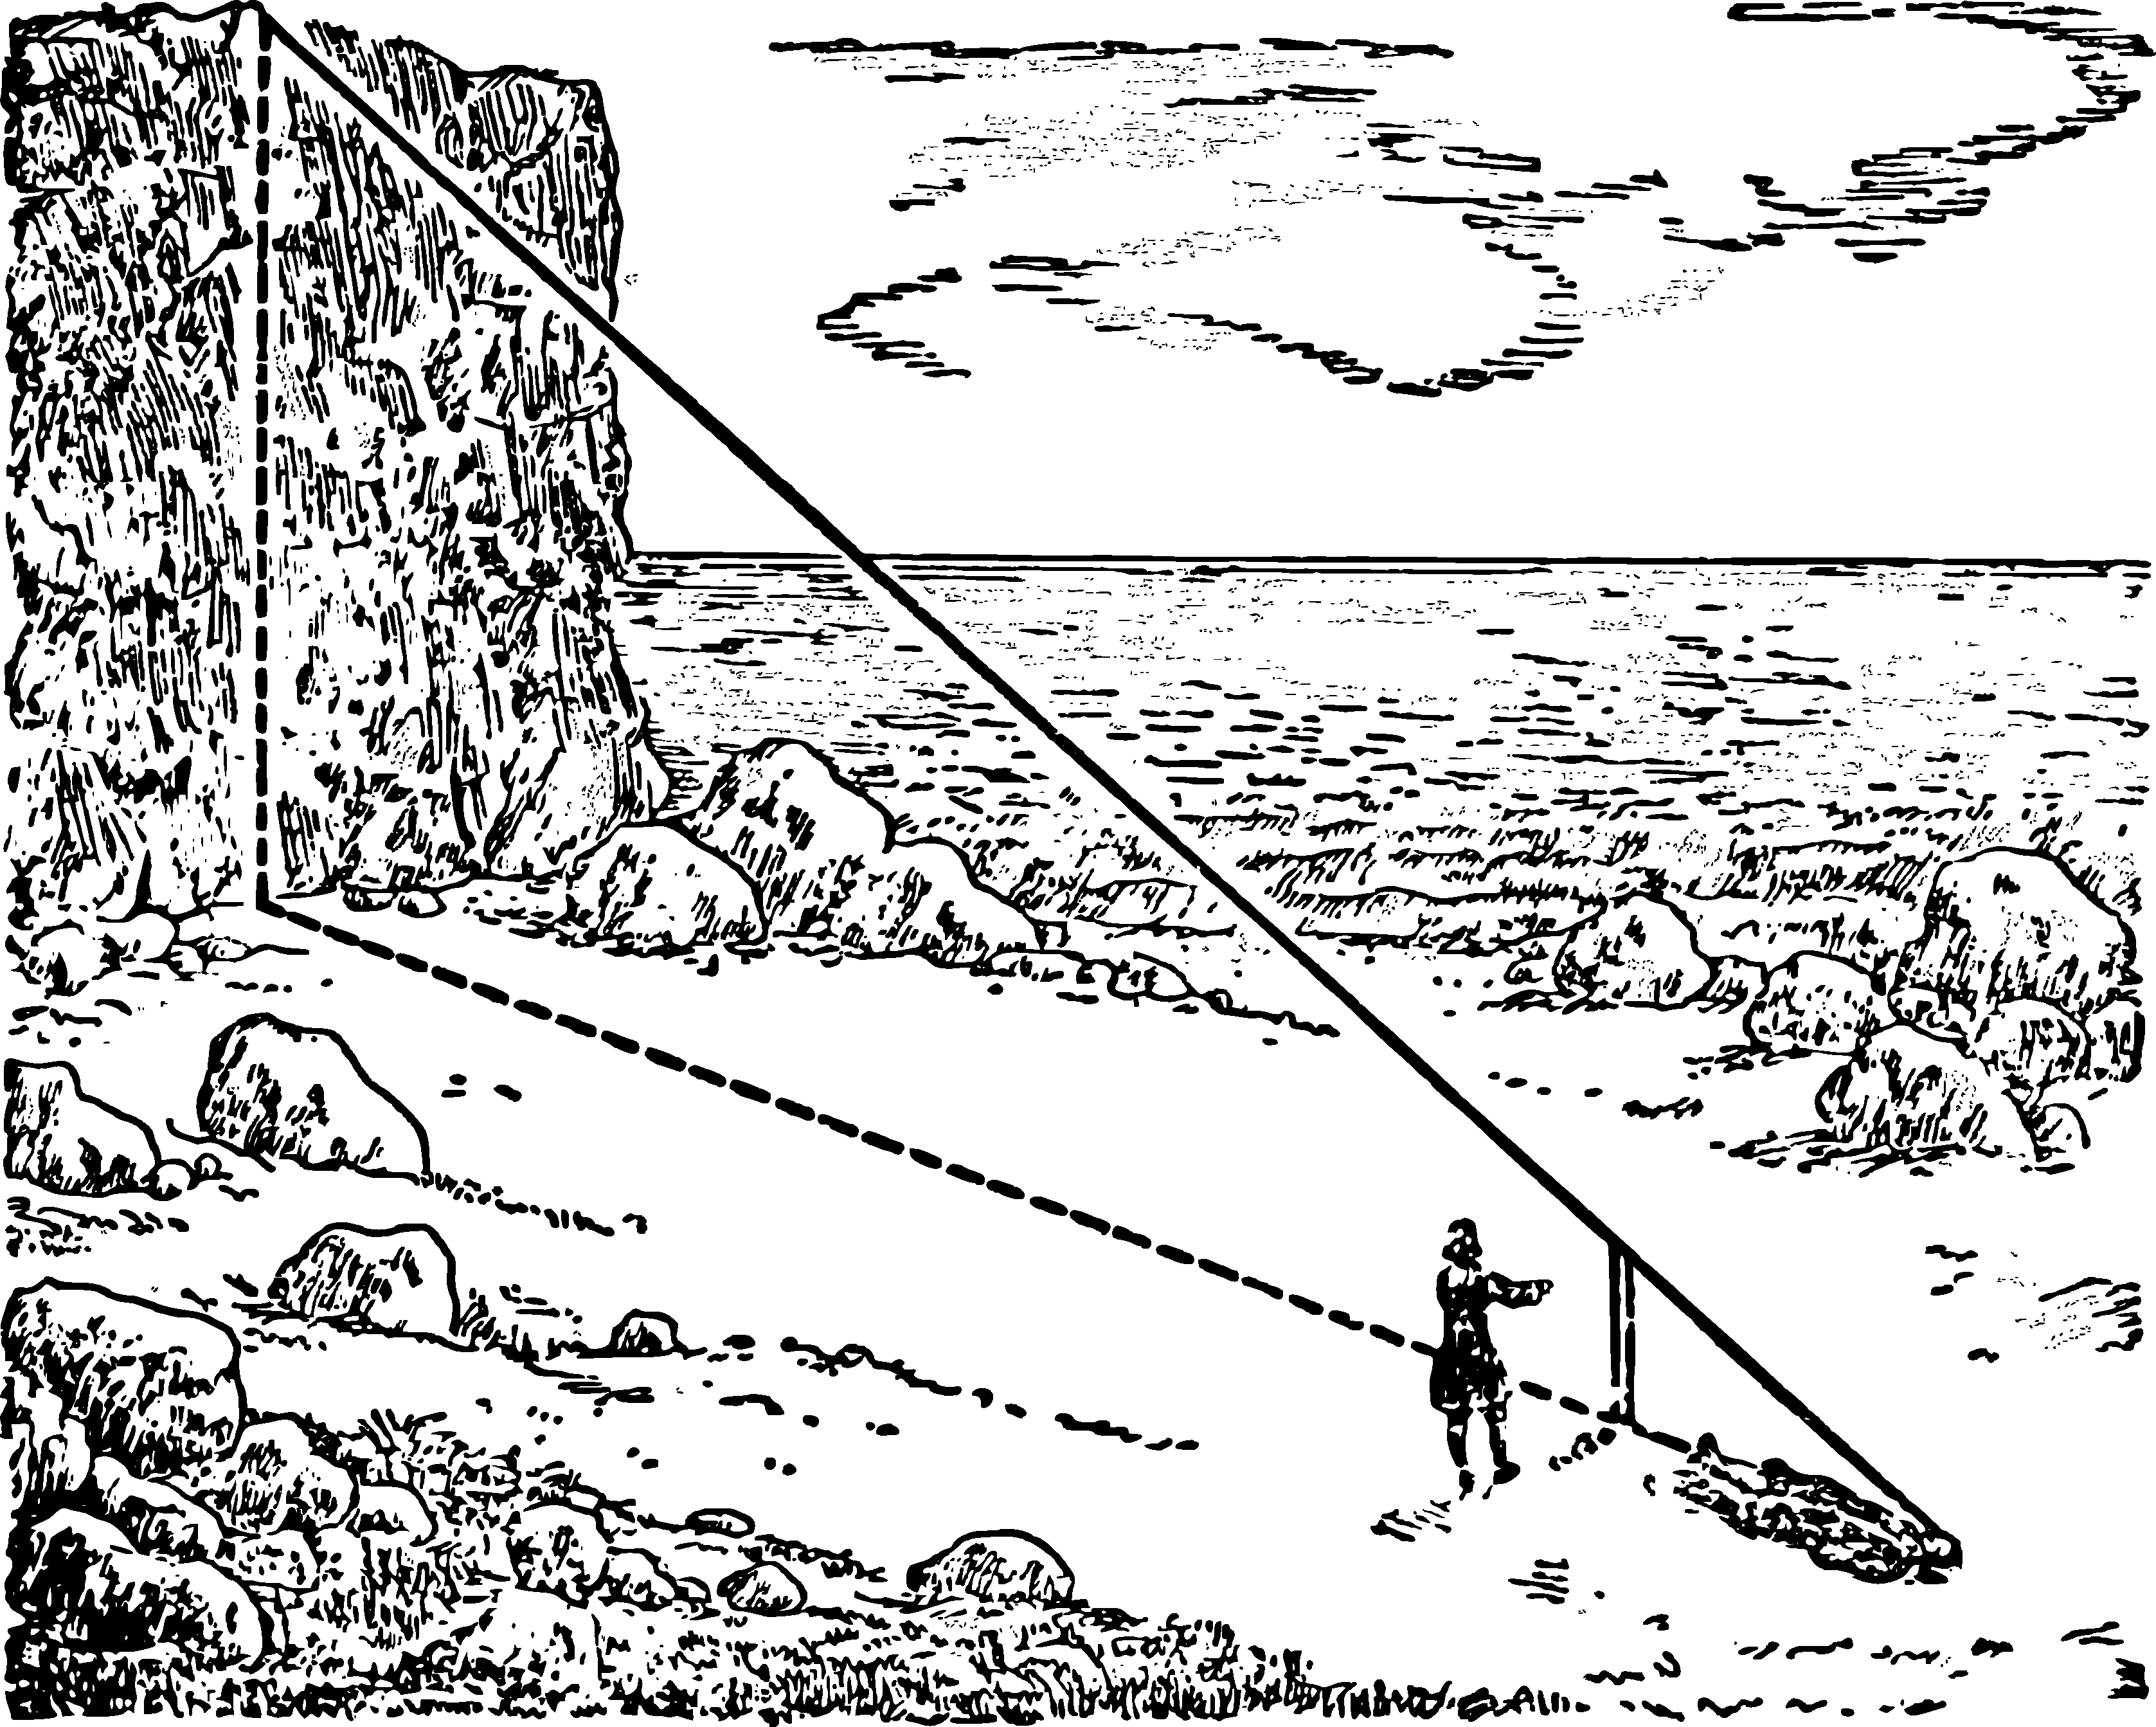
\includegraphics[width=0.9\textwidth]{figures/ch-01/fig-01-07.pdf}
\sidecaption{How the heroes of Jules Verne measured the height of the cliff.\label{fig-01-07}}
\end{figure}

Then he moved away from the pole to a distance where, lying on the sand, one could see both the end of the pole and the edge of the ridge in a straight line (see \figr{fig-01-07}). He carefully marked this point with a stake.

``Are you familiar with the basics of geometry?'' he asked Herbert as he rose from the ground.

``Yes.''

``Do you remember the properties of similar triangles?''

``Their corresponding sides are proportional.''

``Exactly. So now I'll construct two similar right triangles. In the smaller one, one leg will be the plumb-line pole, and the other will be the distance from the stake to the base of the pole; the hypotenuse will be my line of sight. In the other triangle, the legs will be: the granite wall, the height of which we want to determine, and the distance from the stake to the base of this wall; the hypotenuse will be my line of sight, coinciding with the direction of the hypotenuse of the first triangle.''

``Understood!'' exclaimed the youth. ``The distance from the stake to the pole is related to the distance from the stake to the base of the wall, as the height of the pole is to the height of the wall.''

``Yes. And consequently, if we measure the first two distances, then, knowing the height of the pole, we can calculate the fourth, unknown term of the proportion, i.e., the height of the wall. In this way, we can manage without directly measuring the height.''

Both horizontal distances were measured: the smaller one was 15 feet, the larger one was 500 feet.

At the end of the measurements, the engineer made the following record:
\begin{align*}%
15 : 500 & = 10 : x,\\
500 \times 10 & = 5000,\\
5000 : 15 & = 333.3.
\end{align*}
Thus, the height of the granite wall was 333 feet.


\section{How Sergeant Popov Acted}
\label{sec-1.4}

Some of the methods described for measuring height are inconvenient as they require lying on the ground. This inconvenience can, of course, be avoided.

Here's a story from one of the fronts of the Great Patriotic War. Lieutenant Ivanyuk's unit was ordered to build a bridge across a mountain river. On the opposite bank were entrenched fascists. To scout the location for the bridge, the lieutenant assigned a reconnaissance group led by Senior Sergeant Popov. In the nearest forest, they measured the diameter and height of the most typical trees and counted the number of trees that could be used for construction.

They measured the height of the trees using a pole (stick) as shown in \figr{fig-01-08}.

\begin{figure}[h!]
\centering
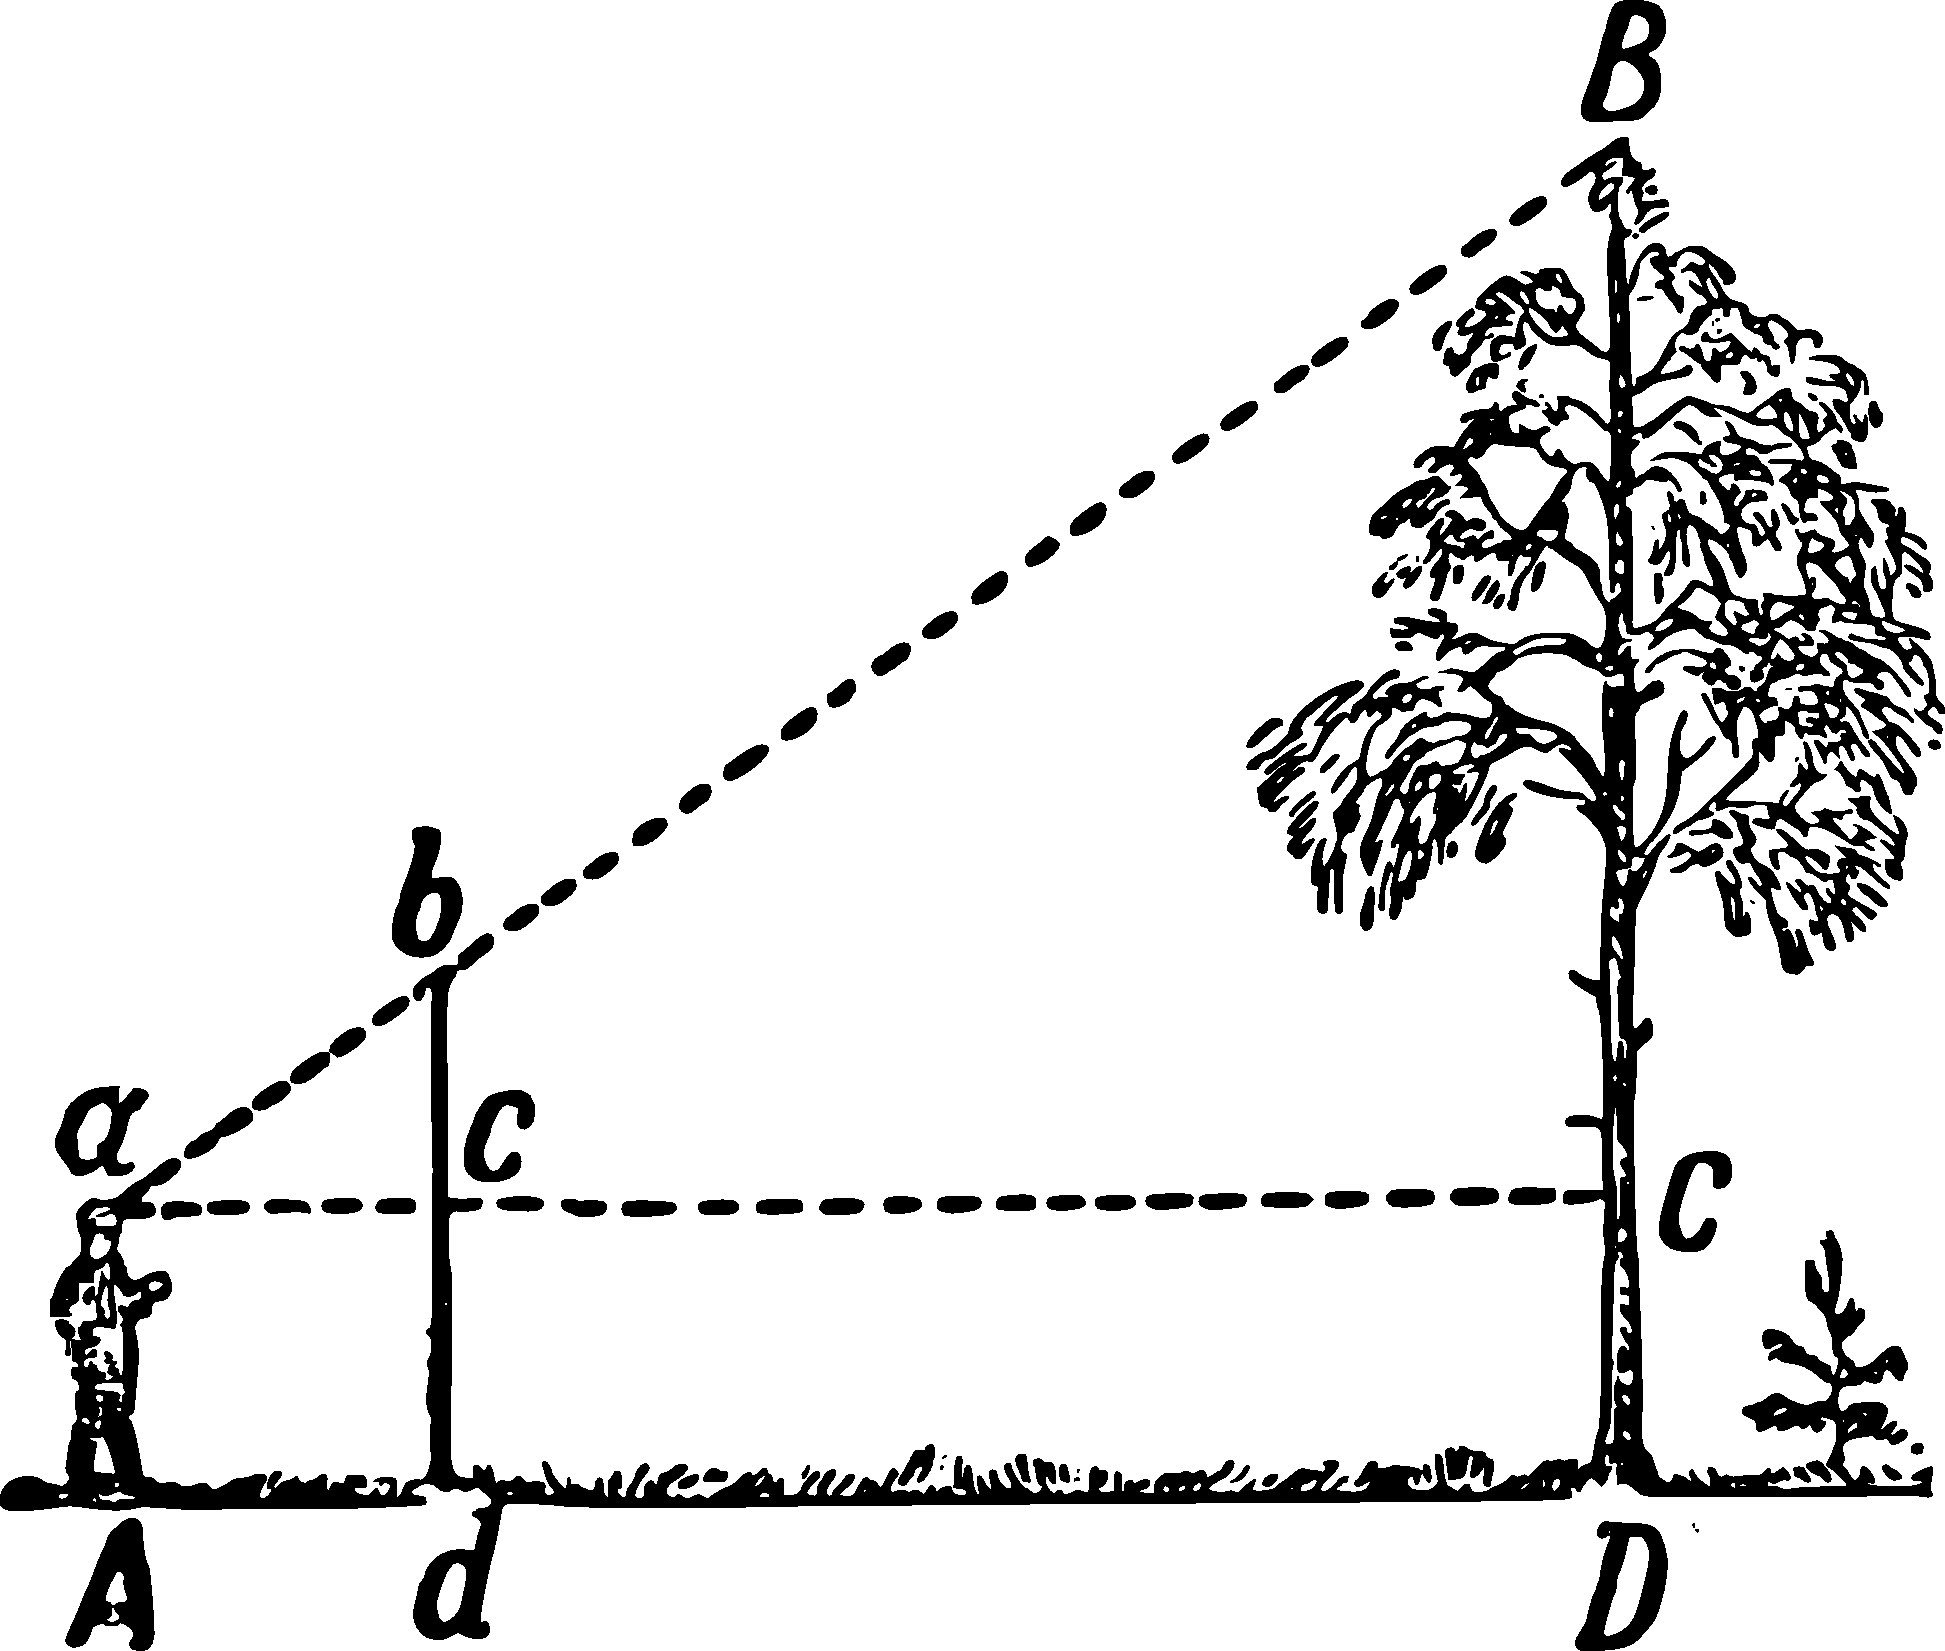
\includegraphics[width=0.6\textwidth]{figures/ch-01/fig-01-08.pdf}
\sidecaption{Measuring the height of the trees with a pole.\label{fig-01-08}}
\end{figure}

This method works as follows: Armed with a pole taller than your own height, drive it into the ground vertically at some distance from the tree being measured (see \figr{fig-01-08}). Step back from the pole along the line $dD$ until you reach point $A$, from where, looking at the top of the tree, you'll see the upper point $B$ of the pole aligned with it. Then, without changing the position of your head, look along the horizontal line $aC$, noting the point $C$ where your line of sight intersects the pole and the tree trunk. Ask your assistant to mark these points, and the observation is complete. Then, based on the similarity of triangles $abc$ and $aBC$, calculate $BC$ from the proportion 
\begin{equation*}%
\frac{BC}{bc} = \frac{aC}{ac},
\end{equation*}
and thus
\begin{equation*}%
BC = bc \cdot \frac{aC}{ac}
\end{equation*}
The distances $bc$, $aC$, and $ac$ can be easily measured directly. To obtain the actual height of the tree, add the distance $BC$ to the distance $CD$, which is also measured directly.

To determine the number of trees, the senior sergeant ordered the soldiers to measure the area of the forest. Then he counted the number of trees in a small area measuring 50 by 50 meters and multiplied accordingly.

Based on all the data collected by the scouts, the unit commander determined where and what kind of bridge needed to be built. The bridge was completed on time, and the combat mission was successfully accomplished!\sidenote{The episodes of the Great Patriotic War described here and further are narrated by A. Demidov in the journal \emph{Military Knowledge} No. 8, 1949, in the article \emph{River Reconnaissance.}}



\section{Using a Notebook}
\label{sec-1.5}

As a device for an approximate estimate of the inaccessible height, you can also use your pocket back book, if it is equipped with a pencil stuck in a cover or a loop with a book. It will help you to build in space those two similar triangles, from which the desired height is obtained. The book should be held near the eyes as shown in the simplified \figr{fig-01-09}. It should be in the vertical book so that, looking from the point $a$, you can see the top of the tree $B$ covered with the tip of the pencil $b$. Then, due to the similarity of the triangles $abc$ and $aBC$, the height of the $BC$ will be determined from the proportion
\begin{equation*}%
\frac{BC}{bc} = \frac{aC}{ac}.
\end{equation*}
The distances of $bc$, $ac$ and $aC$ are measured directly. To the resulting value of the $BC$, add the length of $CD$, which is, on level ground, the height of the eyes above the ground


\begin{figure}[h!]
\centering
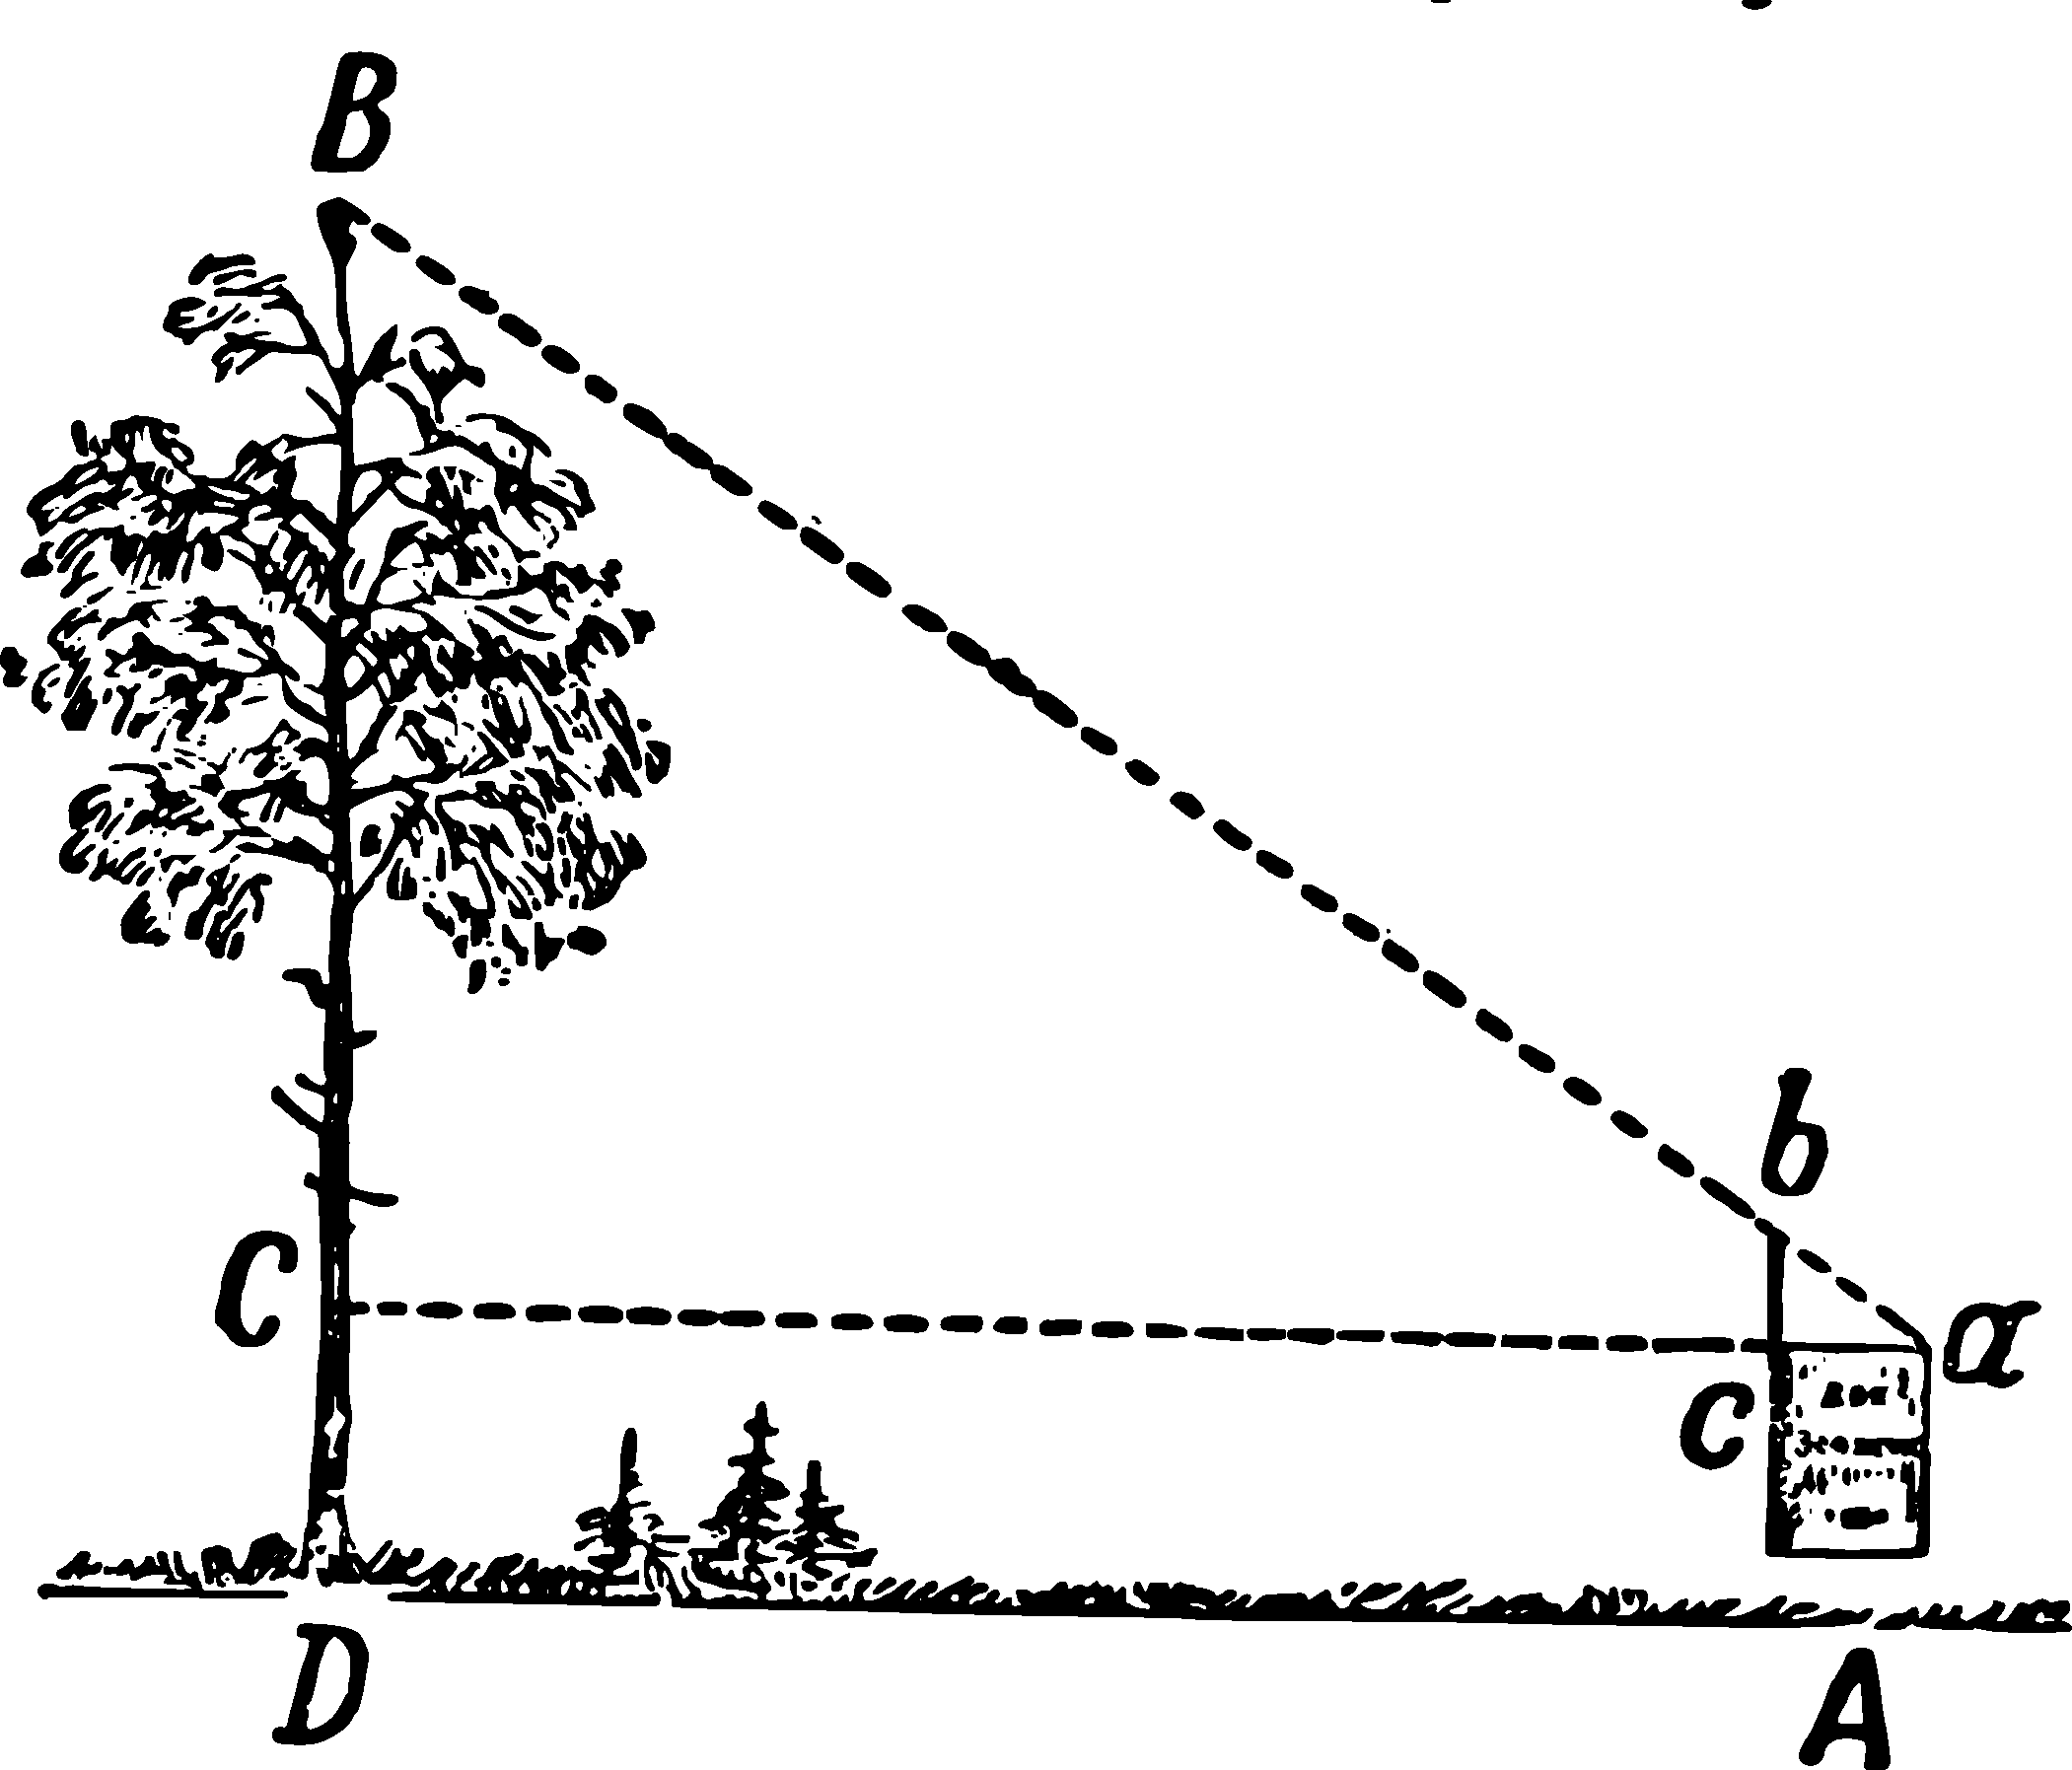
\includegraphics[width=0.6\textwidth]{figures/ch-01/fig-01-09.pdf}
\sidecaption{Height measurement using a notebook.\label{fig-01-09}}
\end{figure}

Since the width of the $ac$ book is unchanged, if you always stand at the same distance from the measured tree (for example, \SI{10}{\meter}), the height of the tree will depend only on the extended part of the pencil. Therefore, you can calculate in advance what height corresponds to a particular extension, and put these numbers on the pencil. Your notebook will then turn into a simplified altimeter, since you can use it to determine heights immediately, without calculations.





\section{Without Approaching The Tree}
\label{sec-1.6}

Sometimes it may be inconvenient to get close to the base of the tree being measured. Can its height still be determined in such a case?

Absolutely. For this purpose, a clever device has been devised, which, like the previous ones, is easy to make by yourself. Two planks, $ab$ and $cd$ (top of \figr{fig-01-10}), are fastened together at right angles so that $ab$ equals $bc$, and $bd$ equals half of $ab$. That's the whole device. 

To measure height with it, hold it in your hands, directing plank CD vertically (for which it has a plumb line with a weight), and stand precisely in two places: first (\figr{fig-01-10}) at point $A$, where the device is positioned with end $c$ up, and then at point $A'$, a bit farther away, where the device is held with end $d$ up. Point $A$ is chosen so that, looking from $a$ to the end of $a$, it is seen on the same line as the top of the tree. Point $A'$ is found so that, looking from $a'$ to point $d'$, it is seen coinciding with $B$. 

The discovery of these two points $A$ and $A'$\sidenote{These points must necessarily lie in a straight line with the base of the tree.} constitutes all the measurement because the desired part of the tree's height, $BC$, is equal to the distance $DA'$. The equality follows easily from the fact that $aC = BC$ and $a'C = 2BC$; thus,
\begin{equation*}%
a'C - aC = BC.
\end{equation*}


\begin{figure}[h!]
\centering
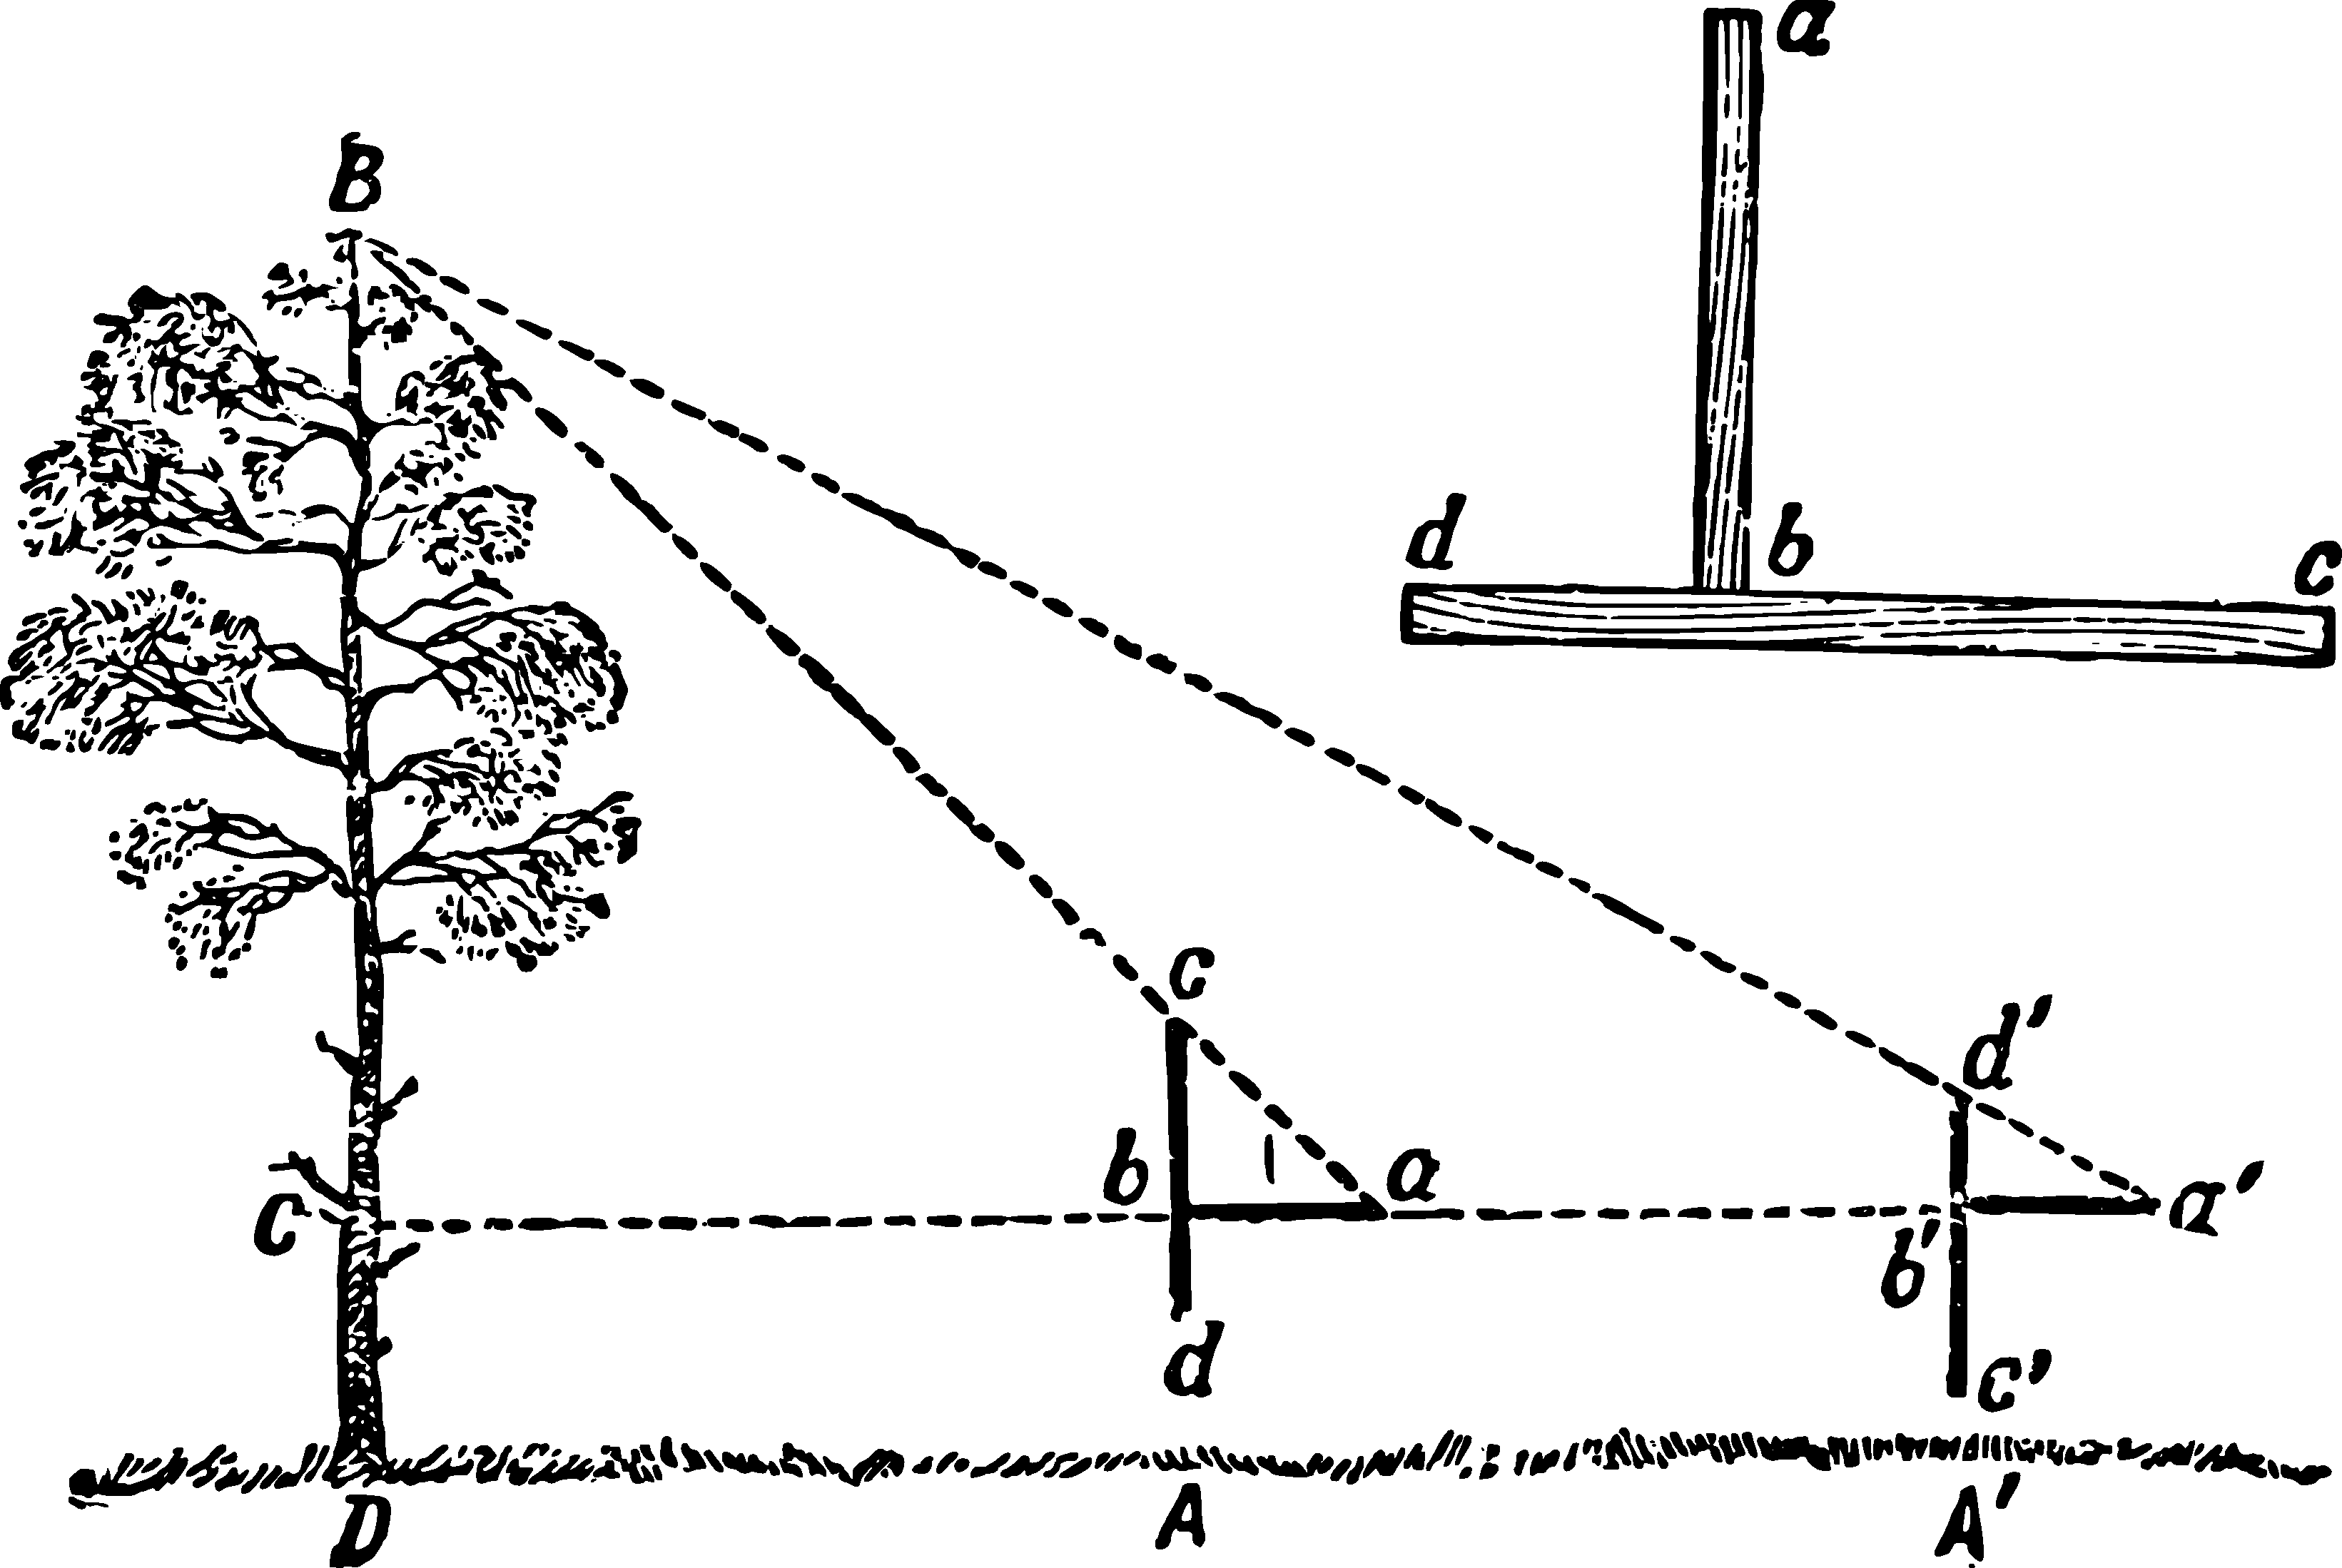
\includegraphics[width=\textwidth]{figures/ch-01/fig-01-10.pdf}
\sidecaption{The use of a simple altimeter consisting of two planks.\label{fig-01-10}}
\end{figure}




You can see that using this simple device, we measure the tree's height without approaching closer than its height. It goes without saying that if it's possible to approach the trunk, it's sufficient to find just one of the points -- $A$ or $A'$ -- to determine its height.

Instead of two planks, you can use four pins, arranging them on a board properly; in this form, the ``device'' is even simpler.

\clearpage

\section{Forest Rangers' Altimeter}
\label{sec-1.7}

It's time to explain how the ``real'' altimeters, used in practise by forest workers, are constructed. I'll describe one of these altimeters, slightly modifying it so that the device can be easily crafted at home. 

\begin{figure}[h!]
\centering
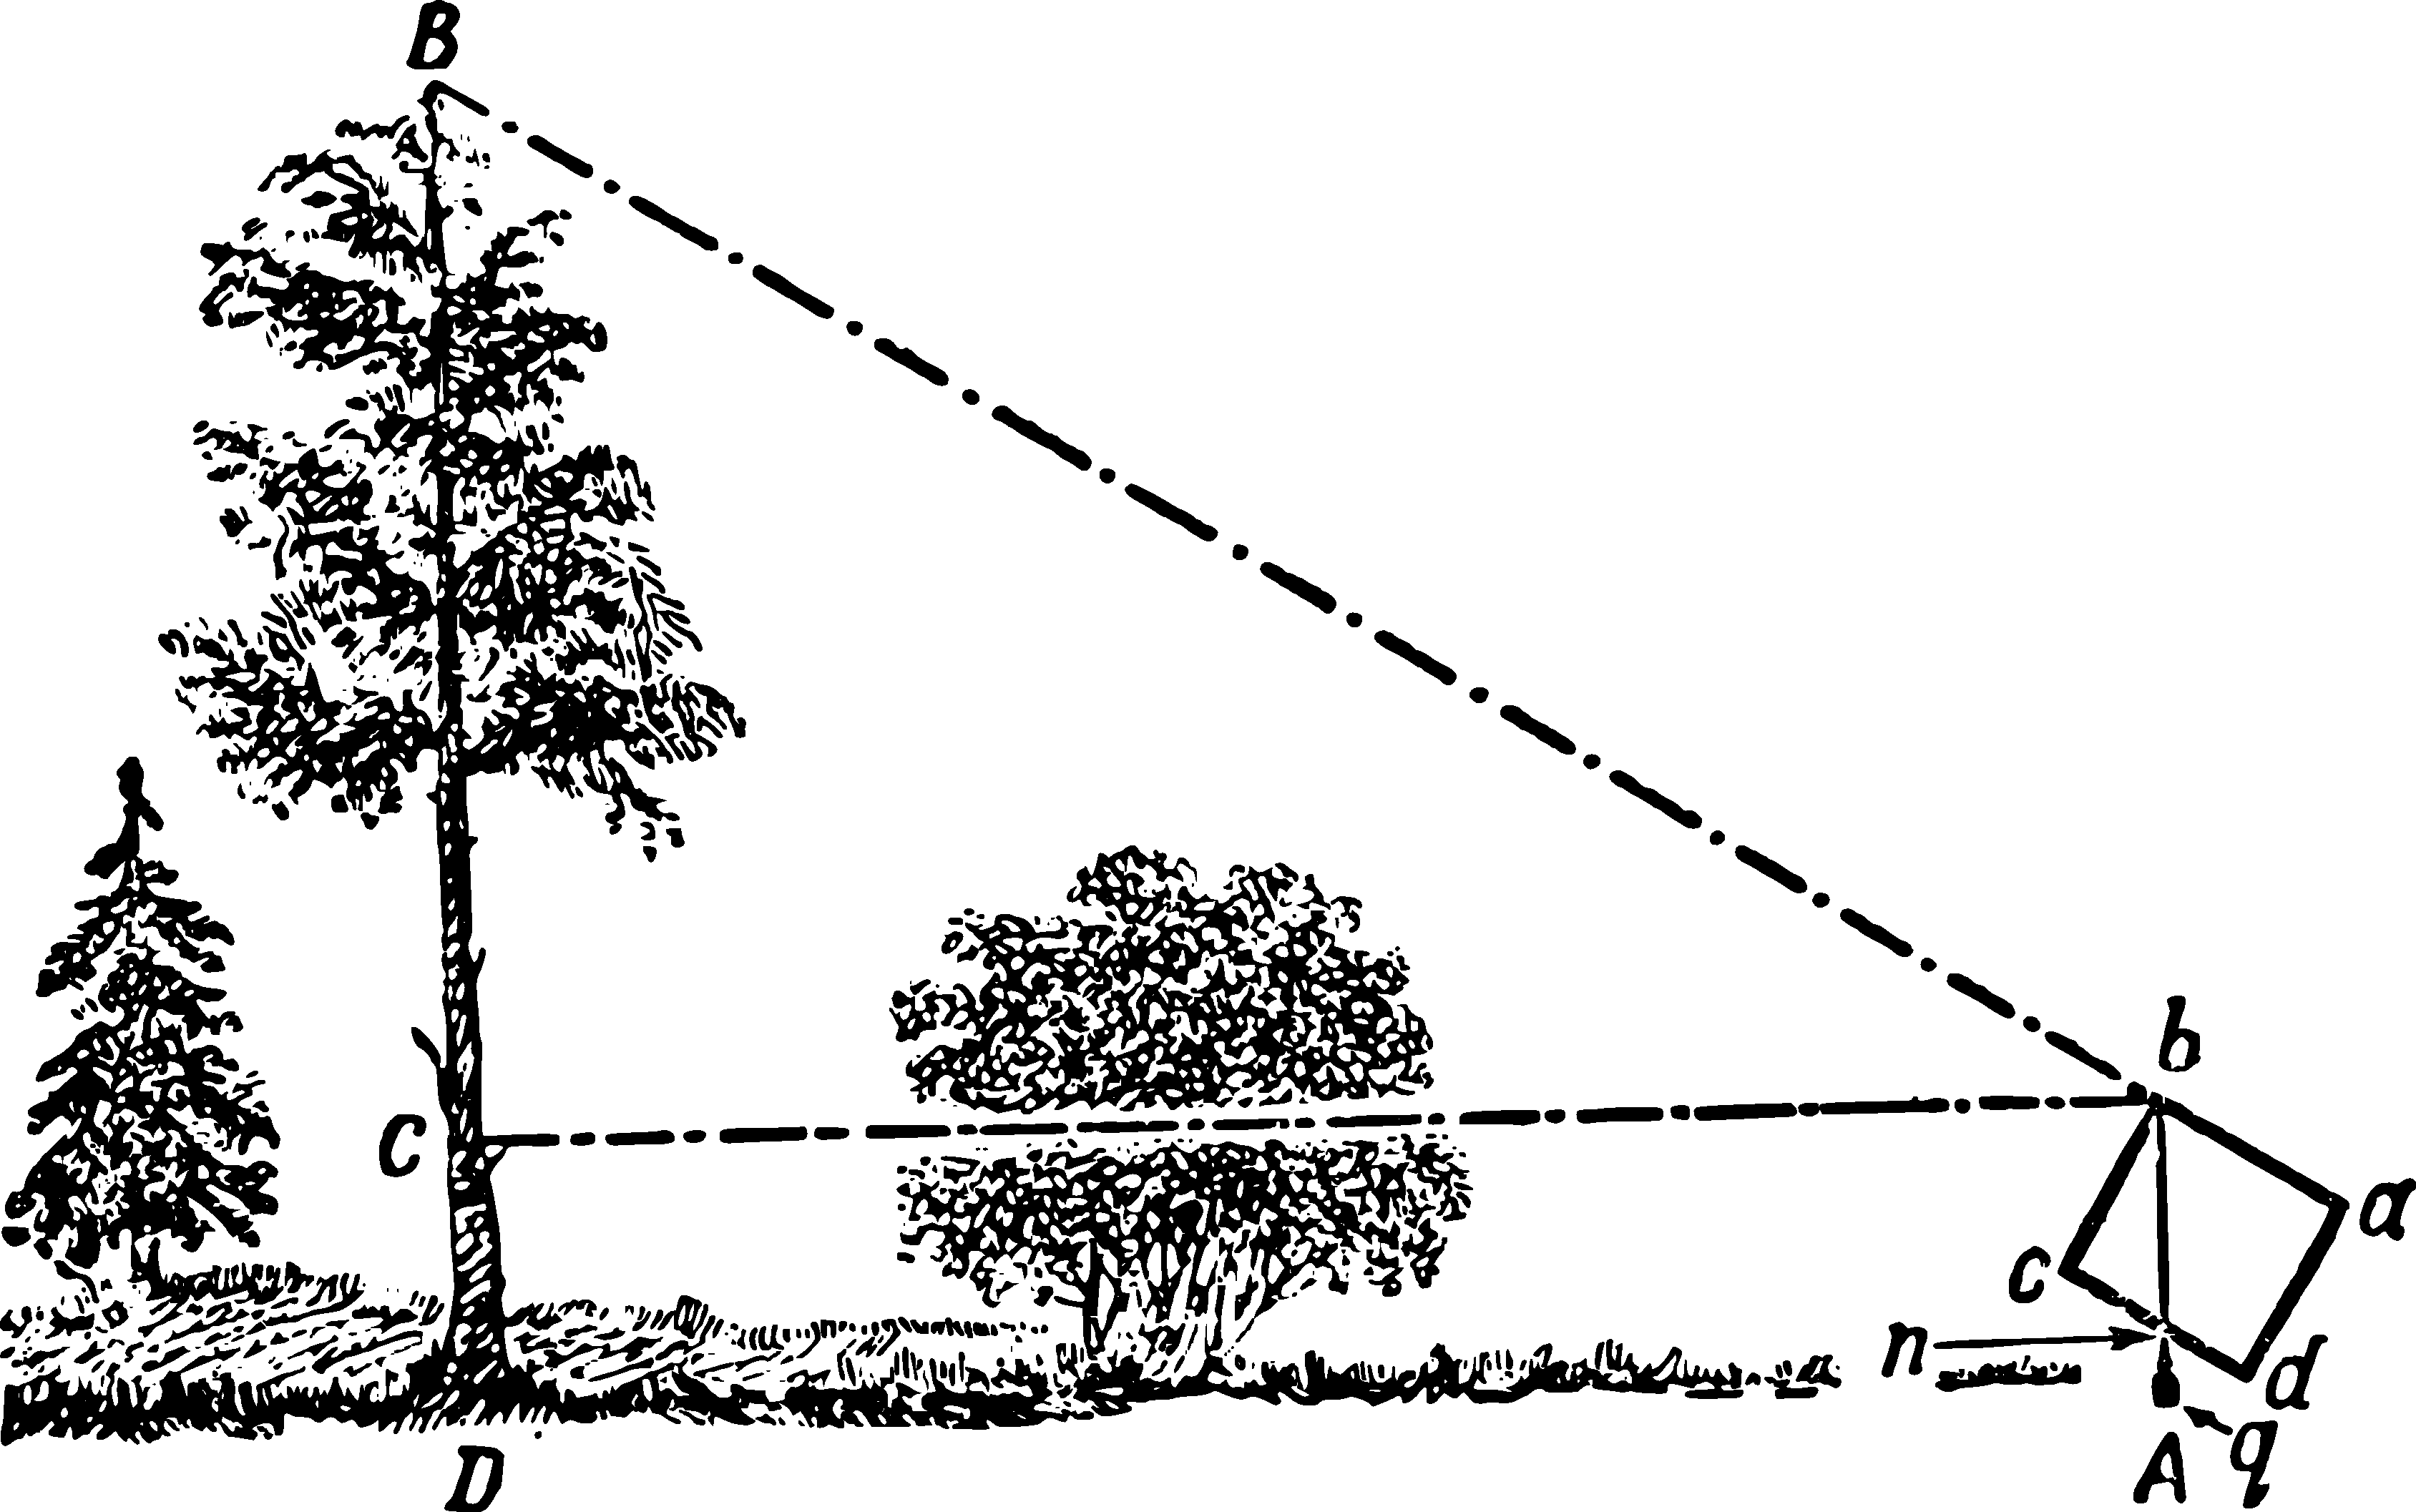
\includegraphics[width=\textwidth]{figures/ch-01/fig-01-11.pdf}
\sidecaption{The scheme of using the altimeter of foresters.\label{fig-01-11}}
\end{figure}


The essence of the device is visible in \figr{fig-01-11}. A cardboard or wooden rectangle, $abcd$, is held in the hand so that, looking along edge $ab$, the tip $B$ of the tree is in line with it. A weight, $q$, is suspended from point $b$ on a thread. We note the point $n$ where the thread intersects line $dc$. Triangles $bBC$ and $bnc$ are similar because they are both rectangular and have equal acute angles $bBC$ and $bnc$ (with corresponding parallel sides). Therefore, we can write the proportion:
\begin{align*}%
\frac{BC}{nc} & = \frac{bC}{bc}; \,\, \text{hence} \\
BC & = bC \cdot \frac{nc}{bc}.
\end{align*}
Since $bC$, $nc$, and $bc$ can be measured directly, it is easy to obtain the desired height of the tree by adding the length of the lower part $CD$ to the trunk (the height of the device above the ground). 

A few details remain to be added. If the edge of the board $bc$ is made, for example, exactly \SI{10}{\centi\meter}, and centimeter divisions are marked on edge $dc$, then the ratio $nc/bc$ will always be expressed as a decimal fraction, directly indicating what fraction of the distance $bC$ represents the height of the tree $BC$. For example, let's say the thread stops against the 7th division mark (i.e., $nc = \SI{7}{\centi\meter}$); this means that the height of the tree above eye level is 0.7 times the observer's distance from the trunk.

\begin{figure}[h!]
\centering
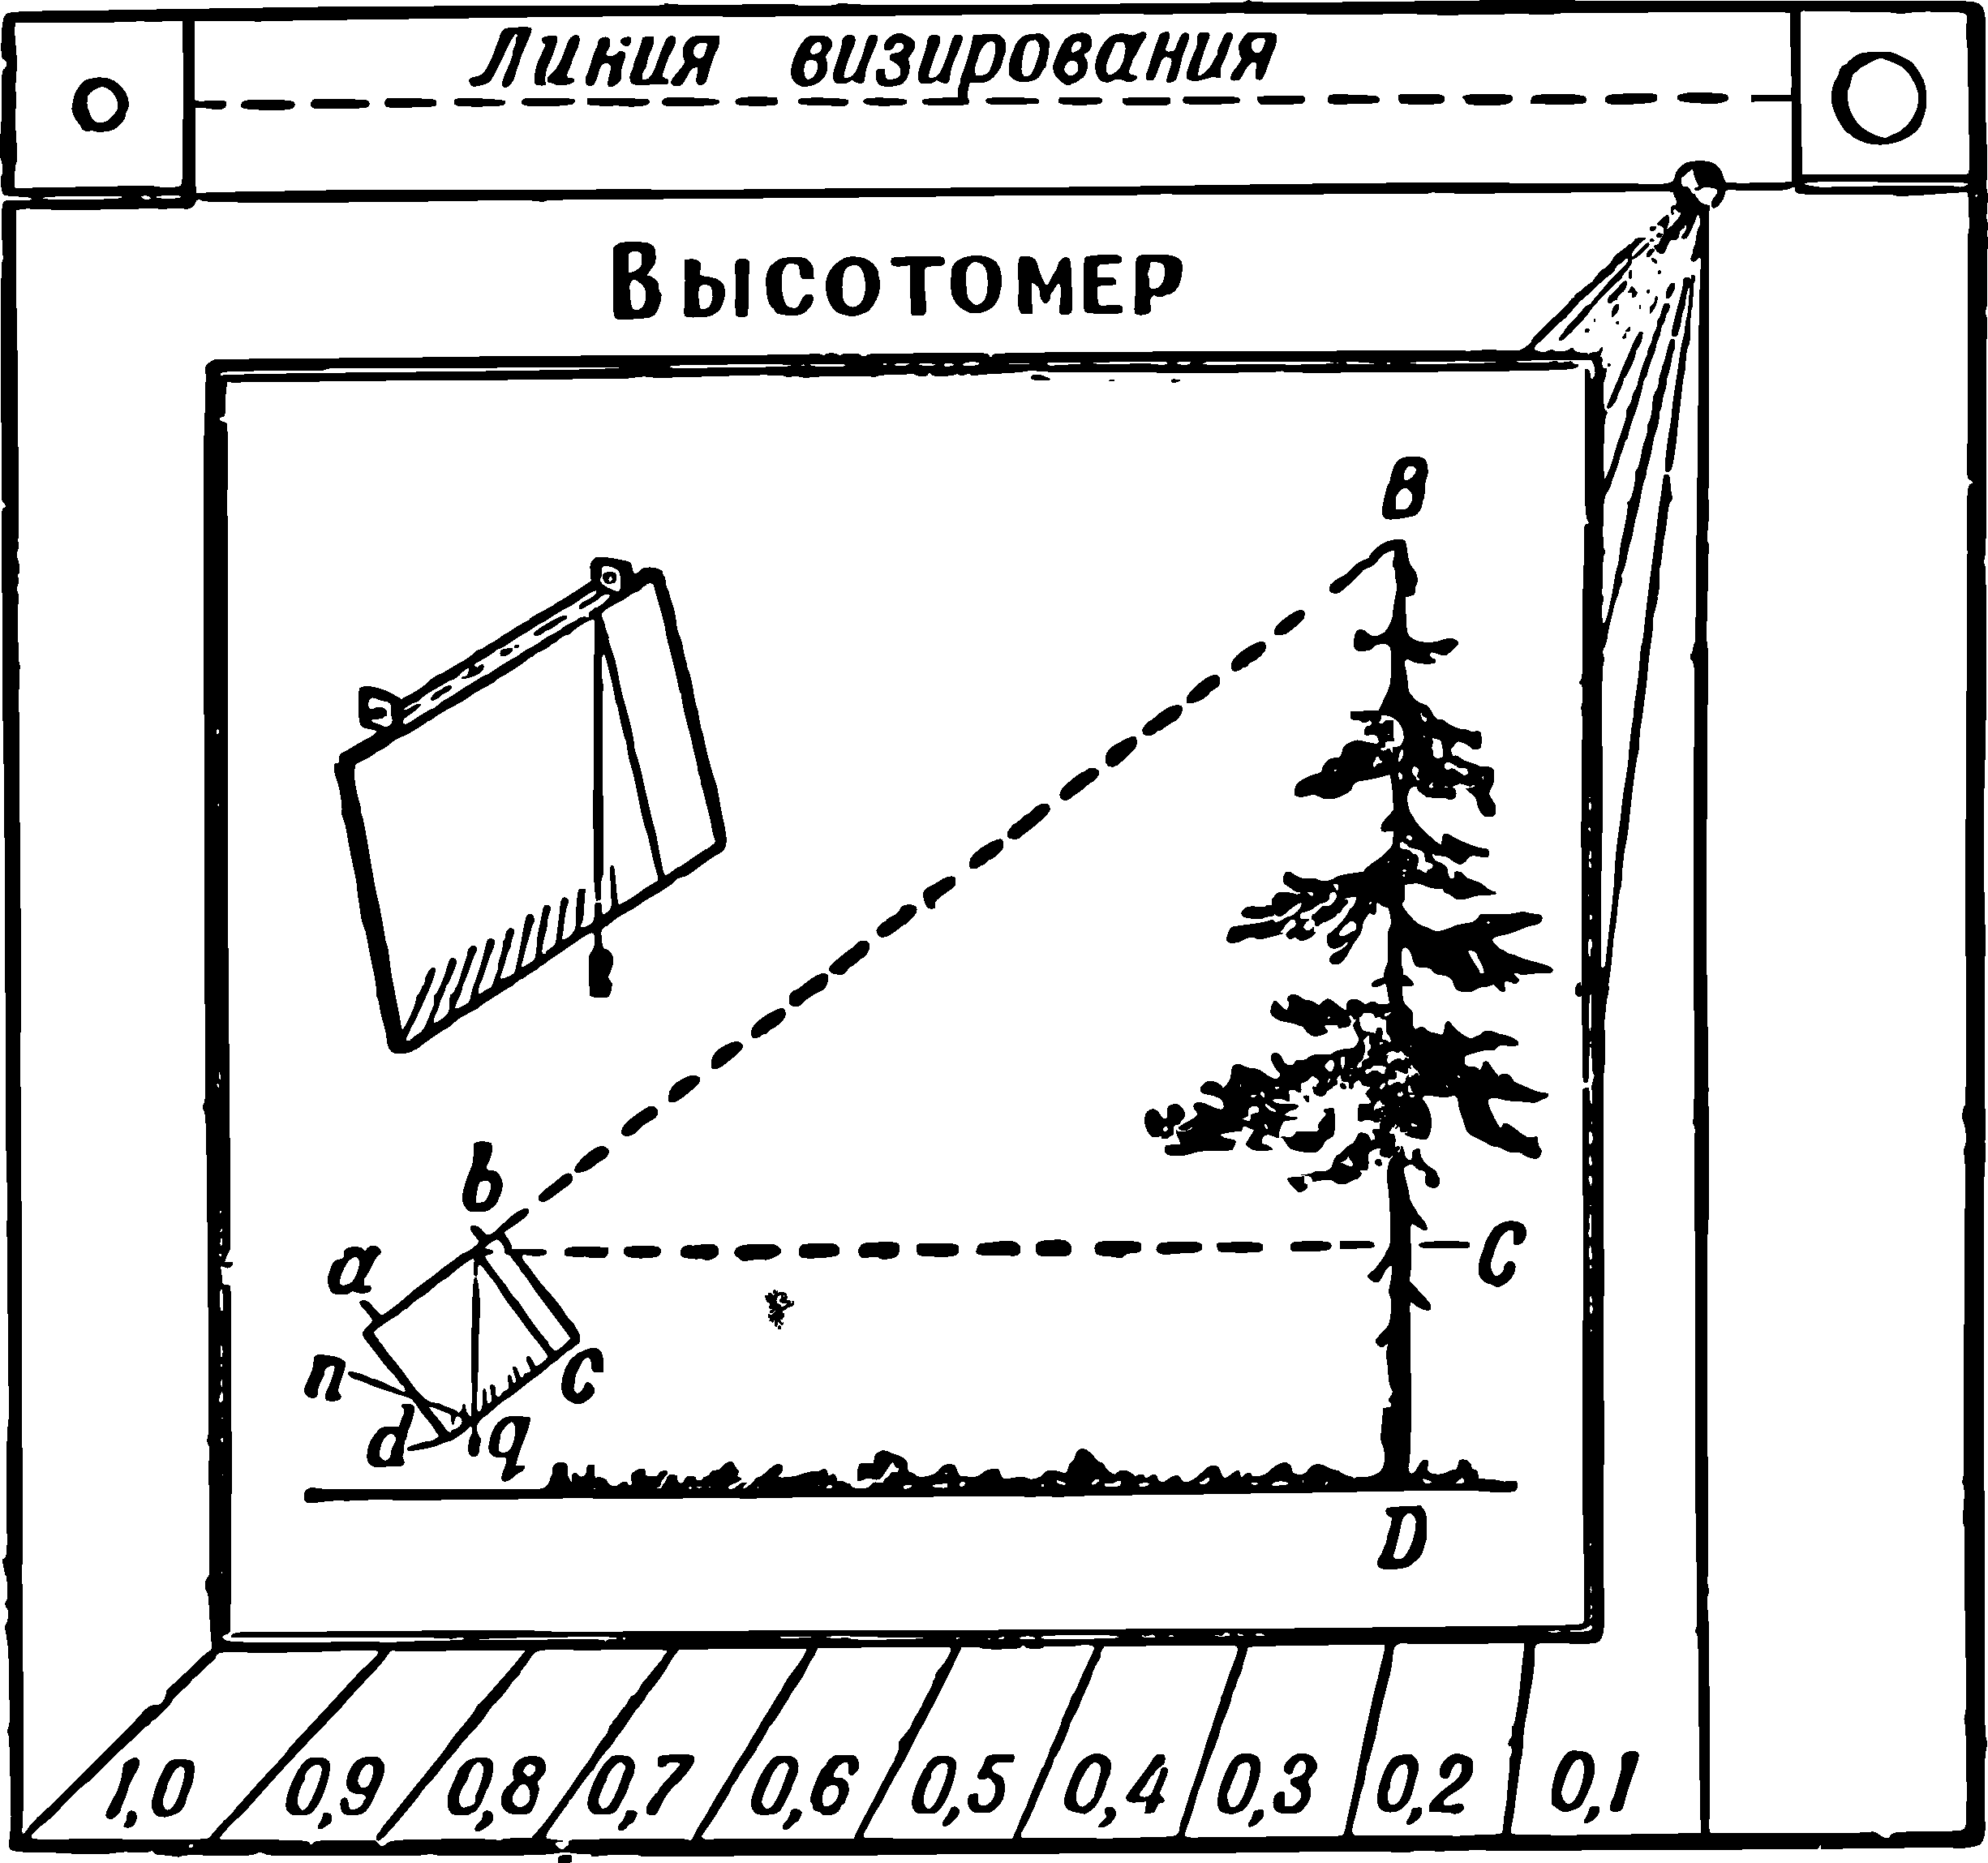
\includegraphics[width=0.7\textwidth]{figures/ch-01/fig-01-12.pdf}
\sidecaption{The forest rangers' altimeter.\label{fig-01-12}}
\end{figure}

The second improvement relates to the method of observation: to make it convenient to look along line $ab$, you can fold down two squares with holes drilled in them at the upper corners of the cardboard rectangle: one smaller one for the eye and one larger one for sighting the tree top (see \figr{fig-01-11}). Further enhancement is represented by the device shown almost to scale in \figr{fig-01-12}. It is easy and quick to make it in this form; no special skill is required. Occupying little space in the pocket, it will provide you with the ability to quickly determine the heights of encountered objects during excursions—trees, poles, buildings, and so on. (This tool is part of the \emph{Geometry in the Open Air} kit developed by the author of this book.)

\subsection*{Question}

Is it possible to use the altimeter described now to measure trees that cannot be approached closely? If possible, what should be done In such cases?

\subsection*{Answer}
The device should be aimed at the top of the tree $B$, as shown in \figr{fig-01-13}, from two points, $A$ and $A'$. 

\begin{figure}[h!]
\centering
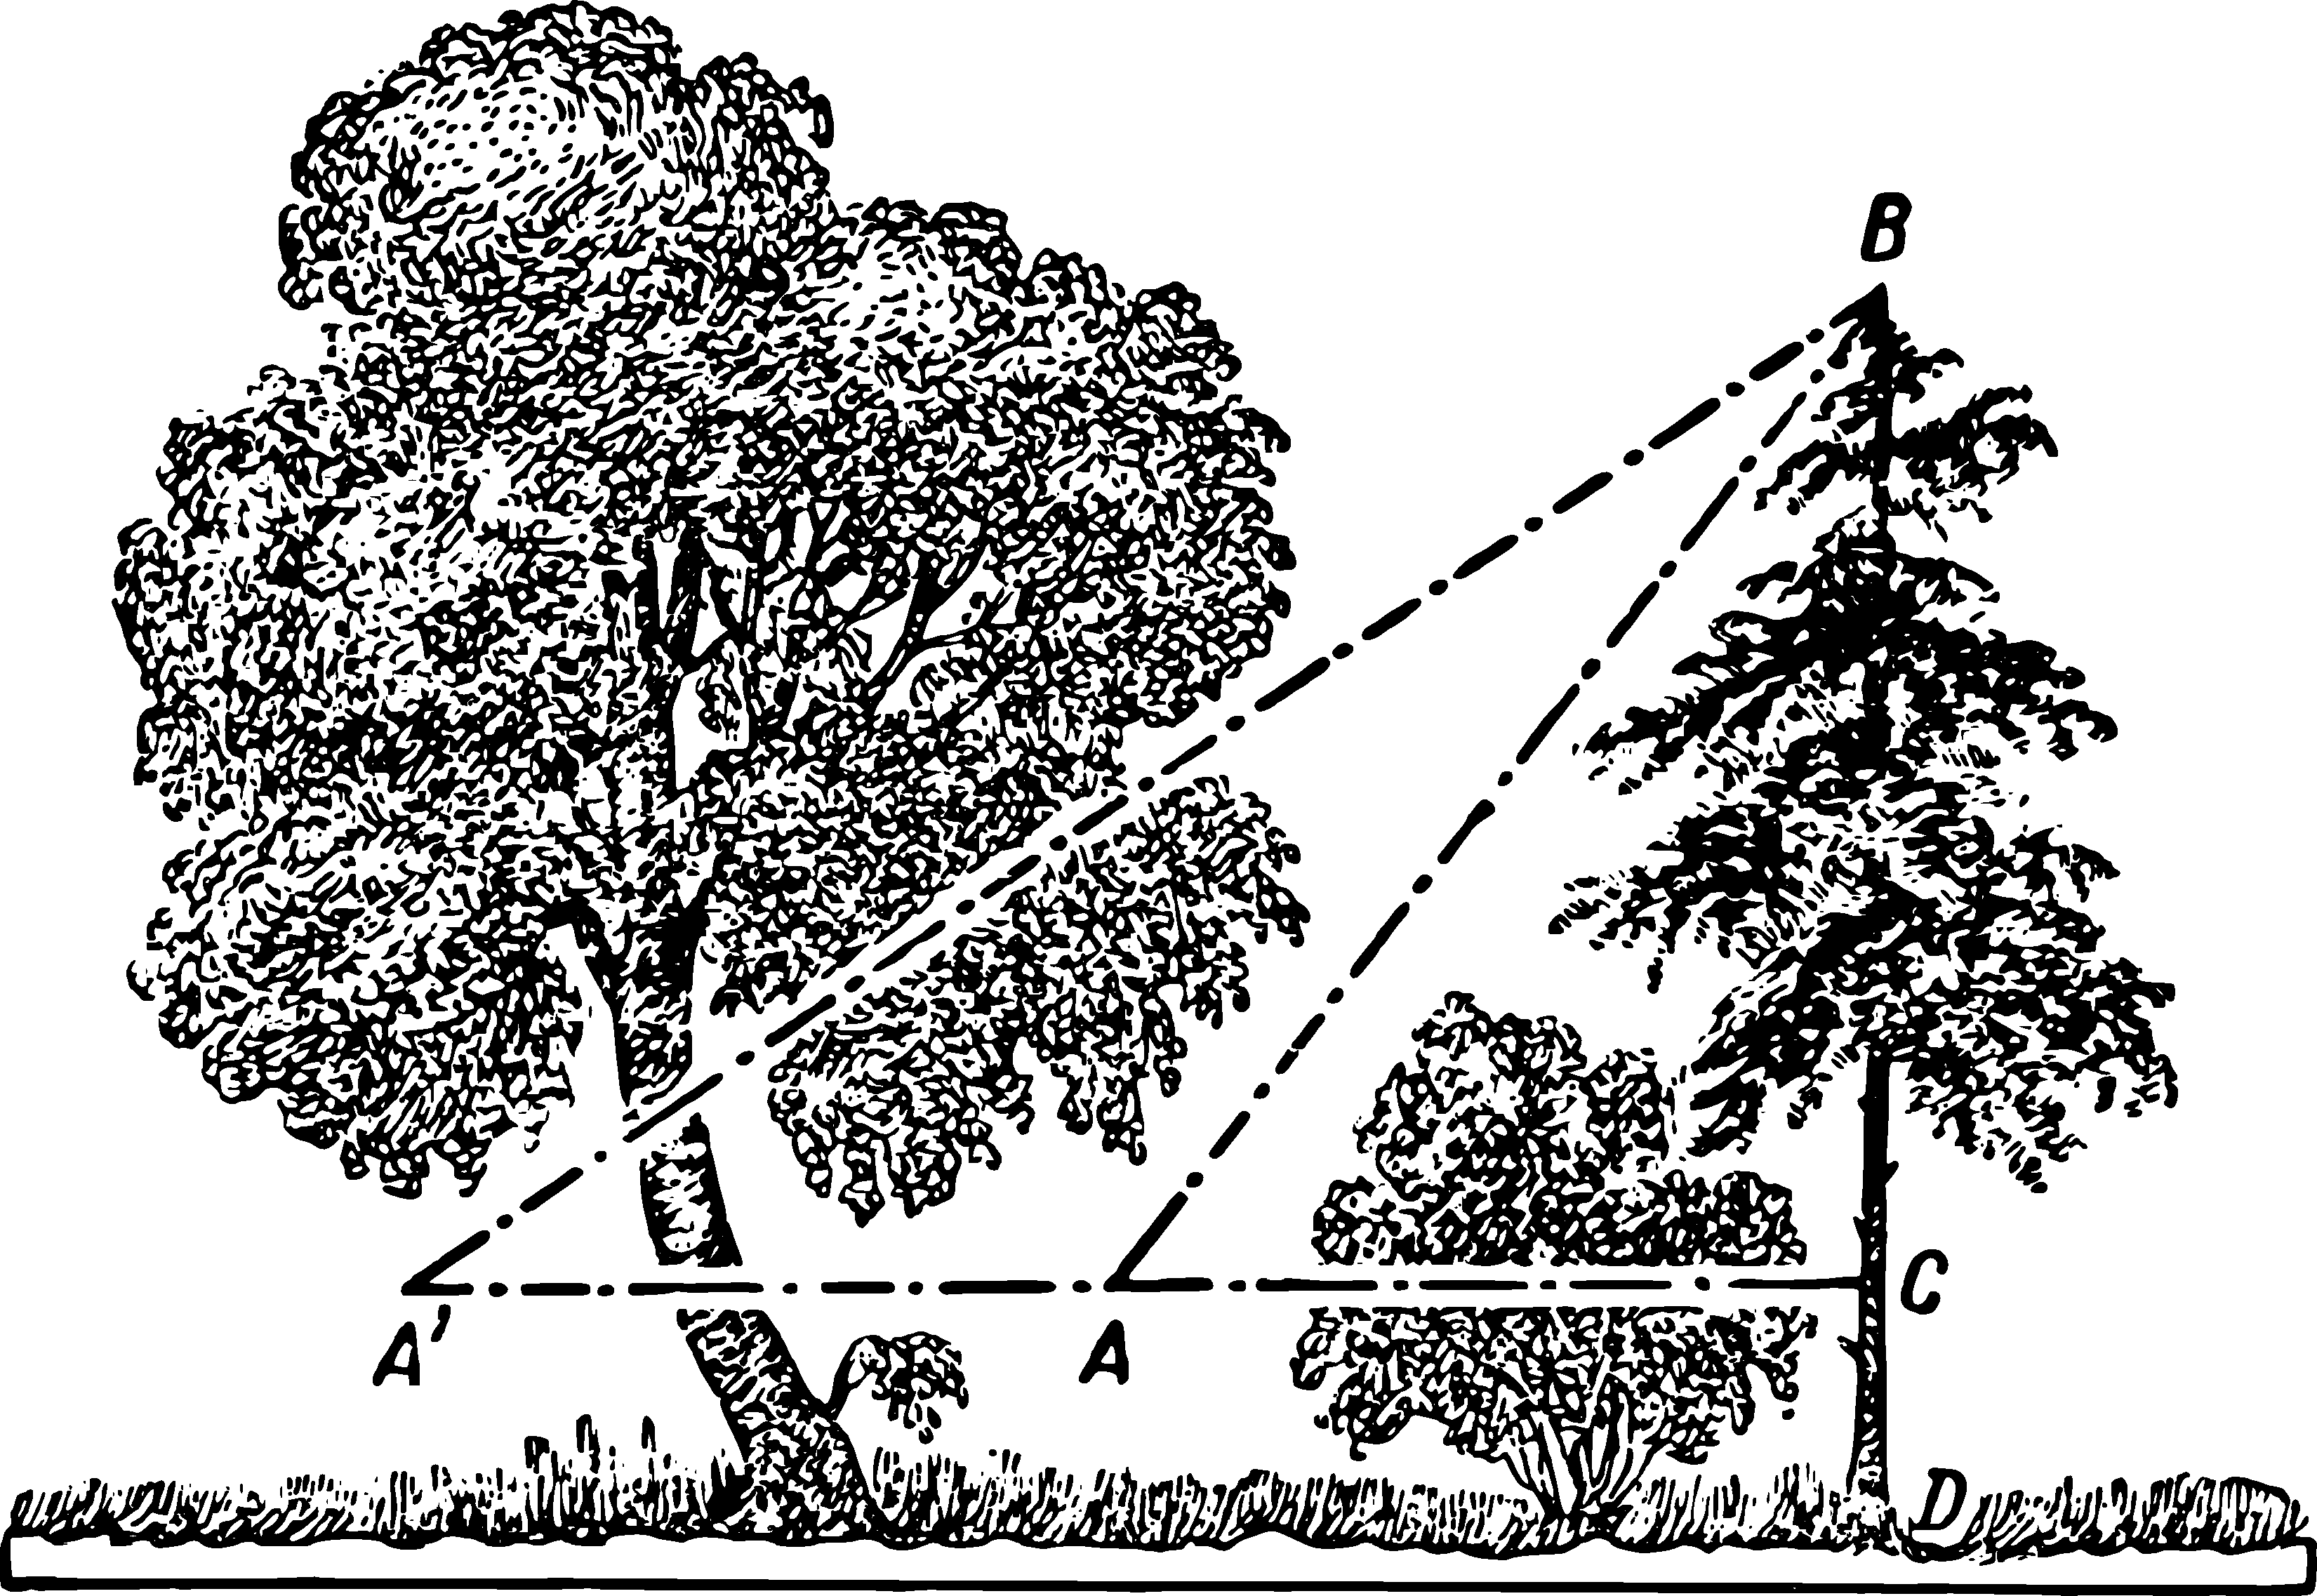
\includegraphics[width=0.9\textwidth]{figures/ch-01/fig-01-13.pdf}
\sidecaption{How to measure the height of a tree without approaching it.\label{fig-01-13}}
\end{figure}

Let's say at point $A$ we determined that $BC = 0.9\,AC$, and at point $A'$ we determined that $BC = 0.4\,A'C$. Then we know that:
\begin{equation*}%
AC = \frac{BC}{0.9},\quad   A'C  = \frac{BC}{0.4} 
\end{equation*}
So that we can write
\begin{equation*}%
AA' = A'C - AC = \frac{BC}{0.4} - \frac{BC}{0.9} = \frac{25}{18} \,BC.
\end{equation*}
Hence,
\begin{align*}%
AA' & = \frac{25}{18} \,BC, \\ 
\therefore BC & = \frac{18}{25} \,AA' \\
& = 0.72 \, AA'.
\end{align*}
You can see that by measuring the distance $AA'$ between both observation points and taking a certain fraction of this value, we can determine the desired and inaccessible height.


